% !TEX program = xelatex
% ============================================================================
% មគ្គុទ្ទេសក៍គរុកោសល្យគ្រូ និងរបាយការណ៍ស្រាវជ្រាវលម្អិត (Teacher's Guideline -- POWQ)
% មុខវិជ្ជា៖ គណិតវិទ្យា ថ្នាក់ទី៨ (ពីជគណិត) -- មេរៀនទី២៖ ស្វ័យគុណ
% ចំណុចរង៖ ២.៤.៣ ស្វ័យគុណនៃផលចែក និងពង្រឹងលក្ខណៈទាំង ៣ (ទំ.១៨, ២៥--២៦)
% គ្រូបង្រៀន៖ ហុក ប៊ុនថែន | អនុវិទ្យាល័យព្រះក្រសាំង (កំពង់ស្វាយ-កំពង់ធំ)
% ============================================================================
\documentclass[a4paper,12pt]{article}

\usepackage[a4paper, left=1.45cm, right=1.45cm, top=2.30cm, bottom=2.30cm, headheight=18pt, headsep=0.68cm, footskip=0.88cm]{geometry}
\usepackage{amsmath, amssymb}
\usepackage{unicode-math}
\usepackage{fontspec}
\usepackage{array, longtable, multirow, colortbl, booktabs}
\usepackage[table]{xcolor}
\usepackage{enumitem}
\usepackage{pifont}
\usepackage{fancyhdr}
\usepackage{lastpage}
\usepackage{needspace}
\usepackage[hyphens]{url}
\usepackage{tikz}
\usepackage[most]{tcolorbox}
\tcbuselibrary{breakable,skins}
\usetikzlibrary{calc, arrows.meta, positioning, decorations.pathreplacing, decorations.markings, patterns, babel}
\urlstyle{same}

\makeatletter
\let\@expl@@@mark@update@singlecol@structures@@\relax
\makeatother

% ============================================================================
% ការកំណត់ពុម្ពអក្សរផ្លូវការ (Cross-Platform Khmer + Times New Roman APA + Cambria Math)
% ============================================================================
\providecommand{\NGSFindFonts}{%
  \IfFileExists{C:/Windows/Fonts/cambria.ttc}{%
    \def\NGSSysPath{C:/Windows/Fonts/}%
    \def\NGSUserPath{C:/Users/KIT/AppData/Local/Microsoft/Windows/Fonts/}%
  }{%
    \IfFileExists{./fonts/KhmerOSsiemreap.ttf}{\def\NGSSysPath{./fonts/}\def\NGSUserPath{./fonts/}}{%
    \IfFileExists{../fonts/KhmerOSsiemreap.ttf}{\def\NGSSysPath{../fonts/}\def\NGSUserPath{../fonts/}}{%
    \IfFileExists{../../fonts/KhmerOSsiemreap.ttf}{\def\NGSSysPath{../../fonts/}\def\NGSUserPath{../../fonts/}}{%
    \IfFileExists{../../../fonts/KhmerOSsiemreap.ttf}{\def\NGSSysPath{../../../fonts/}\def\NGSUserPath{../../../fonts/}}{%
    \IfFileExists{../../../../fonts/KhmerOSsiemreap.ttf}{\def\NGSSysPath{../../../../fonts/}\def\NGSUserPath{../../../../fonts/}}{%
    \IfFileExists{../../../../../fonts/KhmerOSsiemreap.ttf}{\def\NGSSysPath{../../../../../fonts/}\def\NGSUserPath{../../../../../fonts/}}{%
    \IfFileExists{../../../../../../fonts/KhmerOSsiemreap.ttf}{\def\NGSSysPath{../../../../../../fonts/}\def\NGSUserPath{../../../../../../fonts/}}{%
      \def\NGSSysPath{../../../../../../../fonts/}\def\NGSUserPath{../../../../../../../fonts/}%
    }}}}}}}%
  }%
}
\NGSFindFonts

\setmathfont[
  Path={\NGSSysPath},
  FontIndex=1,
  Scale=1.06
]{cambria.ttc}

\defaultfontfeatures{Ligatures=TeX}

\setmainfont[
  Path={\NGSUserPath},
  Extension=.ttf,
  Script=Khmer,
  BoldFont={KhmerOSsiemreap},
  BoldFeatures={FakeBold=1.8},
  ItalicFont={KhmerOSsiemreap},
  ItalicFeatures={FakeSlant=0.25},
  BoldItalicFont={KhmerOSsiemreap},
  BoldItalicFeatures={FakeBold=1.8, FakeSlant=0.25}
]{KhmerOSsiemreap}

% ហាមដាក់ FakeBold លើ KhmerOSmuollight និងកុំរុំ \muol ក្នុង \textbf{...}
% រាល់អក្សរឡាតាំង លេខ ឬសញ្ញា ASCII ក្នុង \muol ត្រូវរុំក្នុង \enbf{...} ឬ $...$
\newfontfamily\muol[
  Path={\NGSUserPath},
  Extension=.ttf,
  Script=Khmer
]{KhmerOSmuollight}

\newfontfamily\TimesEn[
  Path={\NGSSysPath},
  Extension=.ttf,
  Scale=1.02,
  BoldFont={timesbd},
  ItalicFont={timesi},
  BoldItalicFont={timesbi}
]{times}

\newfontfamily\Tacteing[
  Path={\NGSUserPath}
]{TACTENG.TTF}

\newfontfamily\CourierBullet[
  Path={\NGSSysPath},
  Extension=.ttf
]{cour}

% ក្បួនកាត់ពាក្យខ្មែរ (Khmer word wrapping)
\XeTeXlinebreaklocale "km"
\XeTeXlinebreakskip = 0pt plus 1pt minus 0.1pt

% Mobile-First spacing (11.5pt / 18.2pt exact)
\linespread{1.0}

% ============================================================================
% ពណ៌ ស-ខ្មៅ (Strict Monochrome Grayscale Palette) & Fancyhdr
% ============================================================================
\definecolor{headgray}{HTML}{F2F2F2}
\definecolor{panelgray}{gray}{0.94}
\definecolor{stepgray}{HTML}{D9D9D9}
\definecolor{midgray}{gray}{0.82}
\definecolor{bordergray}{gray}{0.45}

\pagestyle{fancy}
\fancyhf{}
\renewcommand{\headrulewidth}{0.4pt}
\renewcommand{\footrulewidth}{0.4pt}
\fancyhead[L]{\rule[-3pt]{0pt}{14pt}\fontsize{9.5pt}{13pt}\selectfont មគ្គុទ្ទេសក៍គរុកោសល្យគ្រូ \en{(Grade 8 POWQ)}}
\fancyhead[R]{\rule[-3pt]{0pt}{14pt}\fontsize{9.5pt}{13pt}\selectfont មេរៀនទី២ \en{(}២.៤.៣\en{)}៖ ស្វ័យគុណនៃផលចែក និងពង្រឹងលក្ខណៈទាំង ៣}
\fancyfoot[L]{\rule{0pt}{13pt}\fontsize{9.5pt}{13pt}\selectfont កញ្ចប់ឯកសារ \en{NGS 5Es (}៥០ នាទី\en{) |} ហុក ប៊ុនថែន}
\fancyfoot[R]{\rule{0pt}{13pt}\fontsize{9.5pt}{13pt}\selectfont ទំព័រ \en{\thepage\ / \pageref{LastPage}}}

\fancypagestyle{firstpage}{%
  \fancyhf{}%
  \renewcommand{\headrulewidth}{0pt}%
  \renewcommand{\footrulewidth}{0.4pt}%
  \fancyfoot[L]{\rule{0pt}{13pt}\fontsize{9.5pt}{13pt}\selectfont កញ្ចប់ឯកសារ \en{NGS 5Es (}៥០ នាទី\en{) |} អនុវិទ្យាល័យព្រះក្រសាំង}%
  \fancyfoot[R]{\rule{0pt}{13pt}\fontsize{9.5pt}{13pt}\selectfont ទំព័រ \en{\thepage\ / \pageref{LastPage}}}%
}

\setlength{\parindent}{0pt}
\setlength{\parskip}{4.5pt}
\setlength{\tabcolsep}{4pt}
\setlength{\emergencystretch}{2em}
\setlist{itemsep=2.8pt, parsep=0pt}

% ============================================================================
% ម៉ាក្រូជំនួយ និងឋានានុក្រម \muol គ្មានតួអក្សរ ASCII បន្លំ
% ============================================================================
\newcommand{\en}[1]{{\TimesEn #1}}
\newcommand{\enbf}[1]{{\TimesEn\textbf{#1}}}
\newcommand{\enit}[1]{{\TimesEn\textit{#1}}}
\newcommand{\unit}[1]{\,\text{\en{#1}}}
\newcommand{\cnum}[1]{{\TimesEn\fontsize{10.5pt}{12pt}\selectfont\ding{\numexpr181+#1\relax}}}
\newcommand{\ditem}{\tikz[baseline=-0.5ex]\fill (0,0.40ex) -- (0.40ex,0) -- (0,-0.40ex) -- (-0.40ex,0) -- cycle;\hspace{0.25em}}
\newcommand{\wcirc}{{\CourierBullet\fontsize{9.8pt}{11pt}\selectfont o}}
\newcommand{\chkbox}{\tikz[baseline=-0.15ex]\draw[black, line width=0.85pt] (0,0) rectangle (0.25cm,0.25cm);}
\newcommand{\khmflourish}{{\Tacteing\fontsize{38pt}{15pt}\selectfont\raisebox{-5pt}{3}}}

\newcommand{\parttitle}[1]{{\muol\fontsize{14pt}{22pt}\selectfont #1}}
\newcommand{\sectitle}[1]{{\muol\fontsize{12pt}{19pt}\selectfont #1}}
\newcommand{\subsectitle}[1]{{\muol\fontsize{11.5pt}{18.5pt}\selectfont #1}}
\newcommand{\tblhead}[1]{{\muol\fontsize{10.2pt}{16pt}\selectfont #1\par}}
\newcommand{\teachersays}[1]{{\muol\fontsize{10.8pt}{17pt}\selectfont «គ្រូនិយាយថា៖} #1»}

\newcolumntype{L}[1]{>{\raggedright\arraybackslash}p{#1}}
\newcolumntype{C}[1]{>{\centering\arraybackslash}p{#1}}
\newcolumntype{R}[1]{>{\raggedleft\arraybackslash}p{#1}}

\newcommand{\secbanner}[2]{%
  \Needspace{2.2cm}%
  \vspace{2pt}%
  \begin{tcolorbox}[
    enhanced, sharp corners, colback=stepgray, colframe=black,
    boxrule=1.1pt, borderline south={0.6pt}{1.8pt}{black},
    top=6pt, bottom=6pt, left=9pt, right=9pt,
    before skip=4pt, after skip=4pt
  ]
    \sectitle{#1}\\[2pt]
    {\fontsize{10pt}{14.5pt}\selectfont\enit{#2}}%
  \end{tcolorbox}%
}

\newcommand{\refbanner}[1]{%
  \Needspace{2.2cm}%
  \vspace{2pt}%
  \begin{tcolorbox}[
    enhanced, sharp corners, colback=headgray, colframe=black,
    boxrule=0.85pt, borderline south={0.6pt}{1.8pt}{black},
    top=6pt, bottom=6pt, left=9pt, right=9pt,
    before skip=4pt, after skip=4pt
  ]
    {\muol\fontsize{12pt}{19pt}\selectfont #1}%
  \end{tcolorbox}%
}

\newcommand{\subsec}[1]{%
  \Needspace{1.7cm}%
  \vspace{3pt}%
  \subsectitle{#1}\par%
  \vspace{-2pt}%
  {\color{black}\hrule height 0.55pt}%
  \vspace{3pt}%
}

\newtcolorbox{phasebox}[3]{%
  enhanced, breakable, sharp corners,
  colback=white, colframe=black,
  boxrule=1.0pt, top=5pt, bottom=5pt, left=9pt, right=9pt,
  toptitle=3.5pt, bottomtitle=3.5pt,
  before skip=5pt, after skip=0pt,
  colbacktitle=headgray, coltitle=black,
  fonttitle=\fontsize{11pt}{17.5pt}\selectfont,
  fontupper=\fontsize{11.5pt}{18.2pt}\selectfont,
  title={%
    \linespread{1.0}\selectfont\renewcommand{\arraystretch}{1.0}%
    \begin{tabular*}{\linewidth}{@{}>{\raggedright\arraybackslash}p{13.55cm}@{\extracolsep{\fill}}r@{}}
      {\muol\fontsize{11pt}{17.5pt}\selectfont #1} & {\fontsize{10.5pt}{15pt}\selectfont\en{#2 |} #3}%
    \end{tabular*}%
  }
}

\newtcolorbox{scriptbox}{%
  enhanced, breakable, sharp corners, colback=panelgray, colframe=black,
  boxrule=0.8pt, borderline west={2.4pt}{0pt}{black},
  top=5pt, bottom=5pt, left=9pt, right=8pt,
  before skip=-0.5pt, after skip=5pt,
  fontupper=\fontsize{11.5pt}{18.2pt}\selectfont
}

\begin{document}
\thispagestyle{firstpage}
\fontsize{11.5pt}{18.2pt}\selectfont
\vspace*{-0.75cm}

% ============================================================================
% ក្បាលលិខិតផ្លូវការថ្នាក់ជាតិ & សាលារៀន (Kampong Thom / Kampong Svay / Preah Krasang)
% ============================================================================
{\linespread{1.08}\selectfont
\begin{center}
  {\muol\fontsize{13.5pt}{21pt}\selectfont ព្រះរាជាណាចក្រកម្ពុជា}\\[2pt]
  {\muol\fontsize{12pt}{18.5pt}\selectfont ជាតិ សាសនា ព្រះមហាក្សត្រ}\\[1pt]
  \khmflourish
\end{center}
\vspace{-4pt}
{\muol\fontsize{10.8pt}{17pt}\selectfont
  មន្ទីរអប់រំ យុវជន និងកីឡា ខេត្តកំពង់ធំ\\
  ការិយាល័យអប់រំ យុវជន និងកីឡា ស្រុកកំពង់ស្វាយ\\
  អនុវិទ្យាល័យព្រះក្រសាំង\par}
\vspace{4pt}
\begin{center}
  \parttitle{មគ្គុទ្ទេសក៍គរុកោសល្យគ្រូ និងរបាយការណ៍ស្រាវជ្រាវ \enbf{(Teacher's Guideline)}}\\[3pt]
  {\fontsize{11.5pt}{18pt}\selectfont\textbf{គណិតវិទ្យា ថ្នាក់ទី៨ \en{(}ពីជគណិត\en{)} \en{---} មេរៀនទី២៖ ស្វ័យគុណ}}\\
  {\fontsize{11.0pt}{17pt}\selectfont\textbf{២.៤.៣ ស្វ័យគុណនៃផលចែក និងពង្រឹងលក្ខណៈទាំង ៣ \en{(}ទំ.១៨, ២៥--២៦\en{)}}}
\end{center}
}

\vspace{2pt}
\begin{tcolorbox}[
  enhanced, breakable, sharp corners, colback=headgray, colframe=black,
  boxrule=0.85pt, top=5pt, bottom=5pt, left=7pt, right=7pt,
  before skip=2pt, after skip=5pt
]
  {\muol\fontsize{11pt}{17pt}\selectfont ព័ត៌មានរដ្ឋបាលមេរៀន \enbf{(Lesson Package Metadata)}}\par\vspace{3pt}
  \linespread{1.0}\fontsize{10.5pt}{15pt}\selectfont
  \renewcommand{\arraystretch}{1.15}
  \begin{tabular}{@{}L{2.85cm}@{}C{0.25cm}@{}L{5.25cm}@{\hspace{0.25cm}}L{2.50cm}@{}C{0.25cm}@{}L{5.65cm}@{}}
    \textbf{\en{-} មុខវិជ្ជា \en{/} ថ្នាក់} & \en{:} & គណិតវិទ្យា ថ្នាក់ទី៨ \en{(}ពីជគណិត\en{)} & \textbf{\en{-} កាលបរិច្ឆេទ} & \en{:} & ថ្ងៃចន្ទ ទី១៦ ខែវិច្ឆិកា ឆ្នាំ២០២៦ \\
    \textbf{\en{-} មេរៀន \en{/} ផ្នែក} & \en{:} & មេរៀនទី២៖ ស្វ័យគុណ \en{(2.4.3)} & \textbf{\en{-} រយៈពេល} & \en{:} & ៥០ នាទី \en{(}១ ម៉ោងសិក្សា\en{)} \\
    \textbf{\en{-} សៀវភៅគោល} & \en{:} & \en{MoEYS} ទំ. ១៧--១៨, ២៥--២៦ & \textbf{\en{-} បង្រៀនដោយ} & \en{:} & ហុក ប៊ុនថែន \en{(NGS} ព្រះក្រសាំង\en{)} \\
    \textbf{\en{-} កញ្ចប់ឯកសារ} & \en{:} & \multicolumn{4}{@{}L{13.90cm}@{}}{ឯកសារ \en{LaTeX} ៤ ច្បាប់ \en{(LS\_Plan, Scenario, Guideline, Printable)} + ថតភស្តុតាង \en{15 Verified OA PDFs}}
  \end{tabular}
\end{tcolorbox}

% ============================================================================
% ផ្នែកទី ១៖ បរិបទមេរៀន និងទិដ្ឋភាពទូទៅនៃកញ្ចប់ឯកសារ ៥ ផ្នែក
% ============================================================================
\secbanner{ផ្នែកទី ១៖ បរិបទមេរៀន និងទិដ្ឋភាពទូទៅនៃកញ្ចប់ឯកសារ ៥ ផ្នែក}{Section 1: Administrative Context, MoEYS Textbook Audit (pp. 17--18, 25--26) \& 5-Part Package Synchronization}

\subsec{១\enbf{.}១ បរិបទអនុវិទ្យាល័យព្រះក្រសាំង និងតួនាទីនៃចំណុចរង ២\enbf{.}៤\enbf{.}៣}

ចំណុចរង \textbf{២.៤.៣ «ស្វ័យគុណនៃផលចែក»} រួមជាមួយ \textbf{ការពង្រឹងលក្ខណៈស្វ័យគុណទាំង ៣} ($(a^m)^n$, $(ab)^n$, និង $\left(\frac{a}{b}\right)^n$) នៅទំព័រ ១៨ និងលំហាត់ជំពូកទំព័រ ២៥--២៦ នៃសៀវភៅគណិតវិទ្យាថ្នាក់ទី៨ ក្រសួងអប់រំ យុវជន និងកីឡា គឺជាចំណុចបញ្ចប់ដ៏សំខាន់នៃផ្នែកលក្ខណៈស្វ័យគុណទាំងមូល។ បន្ទាប់ពីសិស្សបានសិក្សាពី \textbf{២.៤.១} ស្វ័យគុណនៃស្វ័យគុណ និង \textbf{២.៤.២} ស្វ័យគុណនៃផលគុណរួចមក ក្នុងម៉ោងសិក្សានេះ សិស្សត្រូវភ្ជាប់លក្ខណៈទាំង ៣ ជាប្រព័ន្ធតែមួយ ដោយបន្ថែមវិធានស្វ័យគុណនៃផលចែក $\left(\frac{a}{b}\right)^n = \frac{a^n}{b^n}$ (ទាំងទិសផ្ទាល់ ទិសច្រាស និងនិទស្សន្តអវិជ្ជមាន $\left(\frac{a}{b}\right)^{-n} = \left(\frac{b}{a}\right)^n$) មុននឹងបន្តទៅចំណុច \textbf{២.៤.៤ ស្វ័យគុណនៃ ១០} នៅទំព័រ ១៩--២០។

ការពិនិត្យផ្ទៀងផ្ទាត់សៀវភៅសិក្សាគោល (\en{Book pp. 17--18, 25--26}) រួមជាមួយបទពិសោធន៍ថ្នាក់រៀននៅ \textbf{អនុវិទ្យាល័យព្រះក្រសាំង (សាលារៀនជំនាន់ថ្មី \en{NGS})} ស្រុកកំពង់ស្វាយ ខេត្តកំពង់ធំ បង្ហាញពីឧបសគ្គស្នូលចំនួន ៤ យ៉ាងដែលកញ្ចប់ \en{\_POWQ} ត្រូវដោះស្រាយ៖
\begin{itemize}[leftmargin=0.65cm]
  \item \textbf{១. ការភ្លេចលើកស្វ័យគុណភាគបែង និងកំហុសបំប្លែងទម្រង់ច្រាស $\frac{a^n}{b^n} = \left(\frac{a}{b}\right)^n$៖} សិស្សតែងលើកស្វ័យគុណតែភាគយកដោយទុកភាគបែងដដែល ដូចជា $\left(\frac{2}{5}\right)^3 \to \frac{2^3}{5} = \frac{8}{5}$ ឬបូក/ដក/ចែកនិទស្សន្តពេលឃើញ $\frac{9^3}{3^3}$ ជំនួសការផ្គុំជា $\left(\frac{9}{3}\right)^3$។
  \item \textbf{២. អារម្មណ៍បំភាន់លីនេអ៊ែរលើផលបូក និងភាពមិនច្បាស់នៃសញ្ញាដក--វង់ក្រចក៖} សិស្សងាយបំបែកខុសលើផលបូក $\left(\frac{6+4}{2}\right)^2 \to \frac{6^2+4^2}{2^2}$ ព្រមទាំងច្រឡំសញ្ញាដកក្រៅវង់ក្រចក $-2(a^{-3}b^5)^2$ ទល់នឹងក្នុងវង់ក្រចក $\left(\frac{-2}{3}\right)^4$, $\left(\frac{-2x^3}{y^2}\right)^3$ និង $\left(\frac{-3x^2}{y^{-4}}\right)^2$។
  \item \textbf{៣. បន្ទុកការគិត \en{(CLT)} លើកន្សោមចម្រុះមាននិទស្សន្តអវិជ្ជមាន៖} នៅពេលលាយលក្ខណៈទាំង ៣ ជាមួយ $\frac{1}{c^{-n}} = c^n$ ក្នុង $\left(\frac{a^2b^3}{c^{-2}}\right)^3$ ឬ $\left(\frac{-2x^3}{y^2}\right)^3\cdot\frac{y^7}{x^5}$ សិស្សភ្លេចមេគុណលេខ និងផ្លាស់ប្ដូរទីតាំងភាគយក--ភាគបែងខុស។
  \item \textbf{៤. កំណត់សម្គាល់ពុម្ពសៀវភៅគោល (ទំ.១៧--១៨ និង ២៦)៖} នៅ \textbf{ទំព័រ ១៧} ប្រតិបត្តិ ៤.១ ខ. បោះពុម្ព $a\cdot(a^4)^5\cdot a^{-6} = a^{15}$ រីឯនៅ \textbf{ទំព័រ ១៨} ប្រតិបត្តិ ៤.២ ខ. បោះពុម្ពបាត់និទស្សន្តក្រៅ $5$ ក្លាយជា $a\cdot(a^4)\cdot a^{-6} = a^{-1} = \frac{1}{a}$ (ព្រមទាំងខ្វះសញ្ញាចុច «.» ក្រោយអក្សរ «គ» ក្នុង \en{\#8}គ ទំព័រ ២៦)។ គ្រូត្រូវណែនាំការផ្ទៀងផ្ទាត់ទម្រង់ទាំងពីរឱ្យច្បាស់ក្នុងជំហានទី ២។
\end{itemize}

\subsec{១\enbf{.}២ សមាហរណកម្មកញ្ចប់ឯកសារ ៥ ផ្នែក និងផែនទី ៥០ នាទី}

កញ្ចប់ឯកសារ \en{\_POWQ} ទាំង ៥ ផ្នែកត្រូវបានចងក្រងឱ្យស៊ីចង្វាក់គ្នា \en{100\%} ពាក្យ-ទល់-ពាក្យ ទាំងតម្លៃលេខ ធនាគារហេតុផល \cnum{1}--\cnum{5} សញ្ញា [ចង្អុលអូស] កាតវិនិច្ឆ័យ \en{A--D} និងកិច្ចការផ្ទះ៖
\begin{enumerate}[leftmargin=0.65cm]
  \item \textbf{\en{LS\_Plan\_POWQ.tex/.pdf}}៖ កិច្ចតែងការបង្រៀន ៥០ នាទី គំរូ \en{5Es} (\en{2 + 9 + 17 + 20 + $\le$2 min}) សម្រាប់គ្រូអនុវត្តផ្ទាល់ក្នុងថ្នាក់ដោយប្រើជួររងតូចៗងាយអាន។
  \item \textbf{\en{Teaching\_Scenario\_POWQ.tex/.pdf}}៖ សេណារីយ៉ូគ្រប់គ្រងនាទី-ទល់-នាទី ការផ្ទេរតួនាទី ៣ នាក់ ប្លង់ក្ដារខៀន ៣ ផ្នែក និងតារាងវិនិច្ឆ័យកំហុស។
  \item \textbf{\en{Teaching\_Guideline\_POWQ.tex/.pdf}}៖ មគ្គុទ្ទេសក៍គរុកោសល្យបែប \en{Mobile-First} នេះឯង ដែលសំយោគអត្ថបទស្រាវជ្រាវ \en{APA 7th}, ហេតុផលតាមសកម្មភាព, ពាក្យពេចន៍គ្រូនិយាយផ្ទាល់, វិធានការជួសជុលកំហុស, តារាងភស្តុតាង, ចម្លើយគំរូ \en{Pages 1--6} និងបញ្ជីឯកសារយោង។
  \item \textbf{\en{Printable\_Materials\_POWQ.tex/.pdf}} (៦ ទំព័រ \en{A4} ស-ខ្មៅ សុទ្ធ)៖ ១ ឈុតក្នុង ១ ទំព័រ — ទំ. ១ (ក្រឡា \en{1:1} $5\times 5\unit{cm}$, $4\times 4\unit{cm}$ និង \en{Dual POE 2A--2B}), ទំ. ២ (កាតស៊ើបអង្កេត \en{E4} [ចង្អុលអូស]), ទំ. ៣ (សន្លឹក \en{Relay 3} តួនាទី \en{E5}), ទំ. ៤ (ផ្ទាំង \en{Hub-and-Spoke} និងធនាគារ \cnum{1}--\cnum{5}), ទំ. ៥ (កាត \en{Exit A--D} + \en{Exit Ticket} ៣ សំណួរ), ទំ. ៦ (ប័ណ្ណកិច្ចការផ្ទះកាត់ចែក)។
  \item \textbf{ថតភស្តុតាង} ឯកសារស្រាវជ្រាវយោង\_\allowbreak\en{PDF\textbackslash{}}៖ ផ្ទុកឯកសារ \en{Open-Access PDFs} ផ្ទៀងផ្ទាត់រួចចំនួន \textbf{១៥ ច្បាប់} រៀបលេខរៀងពី \en{01\_\allowbreak Fitria2023\_\allowbreak Algebra\allowbreak Misconceptions\allowbreak Map.pdf} ដល់ \en{15\_\allowbreak Yeo2019\_\allowbreak Finger\allowbreak Tracing\allowbreak Worked\allowbreak Examples.pdf} ព្រមទាំង \en{00\_}បញ្ជីឯកសារភស្តុតាង\en{\_\allowbreak Evidence\_\allowbreak Index.md} ដែលត្រូវគ្នា ១-ទល់-១ នឹងផ្នែក \textbf{ឯកសារយោង}។
\end{enumerate}

% ============================================================================
% ផ្នែកទី ២៖ ការសំយោគឯកសារស្រាវជ្រាវអន្តរជាតិ (APA 7th Mini-Literature Review)
% ============================================================================
\secbanner{ផ្នែកទី ២៖ ការសំយោគឯកសារស្រាវជ្រាវអន្តរជាតិ \enbf{(APA 7th Mini-Literature Review)}}{Section 2: Empirical Synthesis of 15 Verified Open-Access Studies Across Three Pedagogical Lenses}

ការរចនាសកម្មភាពបង្រៀនចំណុច ២.៤.៣ និងការពង្រឹងលក្ខណៈទាំង ៣ ត្រូវបានចងភ្ជាប់ដោយផ្ទាល់ទៅនឹងភស្តុតាងវិទ្យាសាស្ត្រ \en{Open-Access} ទាំង \textbf{១៥ ច្បាប់} ដែលសំយោគតាមមុំស្រាវជ្រាវចំនួន ៣ ដូចខាងក្រោម៖

\subsec{២\enbf{.}១ មុំទី ១៖ ការយល់ច្រឡំលើផលចែកស្វ័យគុណ សញ្ញាដក\enbf{-}វង់ក្រចក និងអន្ទាក់លីនេអ៊ែរ}

ការសិក្សាជាក់ស្ដែងបង្ហាញថា ផលចែកស្វ័យគុណ និងនិទស្សន្តអវិជ្ជមានបង្កើតកំហុសធ្ងន់ធ្ងរបំផុតនៅថ្នាក់ទី៨។ \en{Ulusoy (2019)} បានសិក្សាសិស្សថ្នាក់ទី៨ ចំនួន \en{$N = 165$} នាក់ បូករួមនឹងកិច្ចសម្ភាសន៍ \en{$n = 12$} នាក់ ហើយរកឃើញថា មានតែ \en{3.5\% ($n = 4$)} ប៉ុណ្ណោះដោះស្រាយត្រូវទាំង ១០ សំណួរ ខណៈជាង \en{65\%} ទទួលបានពិន្ទុក្រោម \en{3/10}។ ជាក់ស្ដែង លើទម្រង់ផលចែកបញ្ច្រាស \en{Q10} ($\frac{9^3}{3^3} = \left(\frac{9}{3}\right)^3$) មានសិស្សធ្វើត្រូវត្រឹម \textbf{\en{37.6\%}} (\en{34.5\%} ខុស និង \en{27.9\%} ទំនេរ) ដោយច្រឡំដកនិទស្សន្ត $(9/3)^{3-3}=3^0$ (\en{4.8\%}), ដកគោល $(9-3)^3$ (\en{4.2\%}), ឬចែកទាំងគោលទាំងនិទស្សន្ត $(9/3)^{3:3}$ (\en{4.2\%}); រីឯ \en{Q9} ($\frac{5^6}{5^{-3}}$) ធ្វើត្រូវតែ \textbf{\en{17.0\%}} (\en{51.5\%} ខុស ដោយ \en{13\%} ចែកនិទស្សន្ត និង \en{4.2\%} គុណនិទស្សន្ត)។ បន្ថែមលើនេះ សិស្សនៅតែគុណនិទស្សន្តពេលគុណគោលដូចគ្នា (\en{8.4\%} ក្នុង \en{Q6}), បូកនិទស្សន្តពេលបូក (\en{18.1\%} ក្នុង \en{Q4}), គុណគោលនឹងនិទស្សន្ត (\en{4\%}), ខុស $-3^0$ (\en{66.1\%} ខុស; \en{30.9\%} ឆ្លើយ $1$, \en{14.5\%} $-3$, \en{6.6\%} $0$), និងខុស $2^{-4}$ (\en{63.6\%} ខុស; \en{23.6\%} $-16$, \en{13.9\%} $16$)។

ទន្ទឹមគ្នានេះ ការយល់ច្រឡំពីសញ្ញាដក វង់ក្រចក និងការចែកចាយខុសលើផលបូកត្រូវបានបញ្ជាក់ដោយការសិក្សាចំនួន ៤ បន្ថែមទៀត៖
\begin{itemize}[leftmargin=0.65cm]
  \item \textbf{ភាពមិនច្បាស់នៃសញ្ញាដក និងវង់ក្រចក (\en{Olson et al., 2011})៖} ការស្ទង់មតិលើ \en{$N = 904$} នាក់ (\en{>40\%} ខុសលើ ៤/១៩ សំណួរ) និងសម្ភាសន៍ \en{$n = 19$} នាក់ រកឃើញថា ពេលប្រៀបធៀប $(-17)^8$ និង $-17^8$ មានតែ \en{5/19} នាក់ (\en{26.3\%}) ឆ្លើយត្រូវ ខណៈ \en{6/19} នាក់ (\en{31.6\%}) អះអាងថា \textit{«វង់ក្រចកមិនសំខាន់»} ដោយចាត់ទុក $-17$ និង $(-17)$ ជាវត្ថុតែមួយ ជំនួសការមើលឃើញ $-1 \times 17^8$ និងខ្វះគោលគំនិតច្រាសគុណលើ $n^{-1}$។ កំហុសនេះគំរាមកំហែងផ្ទាល់ដល់កំណែ $-2(a^{-3}b^5)^2$, ប្រតិបត្តិ $\left(\frac{-2}{3}\right)^4$, សំយោគ $\left(\frac{-2x^3}{y^2}\right)^3$, និងកាត \en{Exit D} ($-9x^4y^8$)។
  \item \textbf{ការបំផ្លើសច្បាប់ចែកចាយលើផលបូក (\en{Fitria et al., 2023; Kshetree et al., 2021})៖} \en{Fitria et al. (2023)} លើសិស្សថ្នាក់ទី៨ \en{$N = 68$} នាក់ (អាយុ ១៣--១៤ ឆ្នាំ) រកឃើញថា \en{45/68 (66.2\%)} មានកំហុសវិនិច្ឆ័យ (\en{20.8\%--58.3\%}) រួមទាំងការប្រើច្បាប់បំបែក $a(b+c)=ab+ac$ ខុសកន្លែងទៅលើស្វ័យគុណ $(5+x)^2 \to 5^2+x^2$ ដោយ \textit{«ប្រើវិចារណញាណសុទ្ធ»}។ ស្របគ្នានេះ \en{Kshetree et al. (2021)} លើសិស្សថ្នាក់ទី៨ \en{$N = 80$} នាក់ (\en{$n = 37$} ពិសោធន៍ \en{vs} \en{$n = 43$} ត្រួតពិនិត្យ; សម្ភាសន៍ \en{$n = 24$}; \en{split-half 0.731, Spearman-Brown 0.844}) រកឃើញកំហុស $(x+y)^n = x^n+y^n$, $(-x)^2 = -x^2$, $x^2\cdot x^4 = x^8$ ហើយបញ្ជាក់ថា វិធីបង្រៀនផ្ដោតលើជម្លោះគំនិត និងកិច្ចពិភាក្សាក្រុមឈ្នះក្រុមប្រៀបធៀបយ៉ាងច្បាស់ (\en{$U = 1194.000, Z = 3.859, p = .000, r = 0.431$}; ផ្នែក \en{Conceptual $r = 0.383$, Procedural $r = 0.458$, Application $r = 0.405$})។
  \item \textbf{ការព្រមានមិនឱ្យភ័យខ្លាចការចែកចាយត្រឹមត្រូវ (\en{Van Dooren et al., 2003})៖} ពិសោធន៍ថ្នាក់ទី៨ \en{$N = 35$} នាក់ (\en{$n = 18$} \en{vs} \en{$n = 17$}) បង្ហាញថា ទោះបីការបង្រៀនជំទាស់លើកកម្ពស់លំហាត់មិនមែនលីនេអ៊ែរ (\en{29.2\% $\to$ 61.1\%}, \en{$t(488) = 3.09, p = .0001$}; \en{ANCOVA posttest 44.3\% vs 22.3\%}, \en{$F(1,32) = 6.42, p = .0164$}) ក៏ដោយ ក៏ភាពត្រឹមត្រូវលើទម្រង់សមាមាត្រពិតបានធ្លាក់ចុះ (\en{83.3\% $\to$ 58.3\%}, \en{$t(488) = -2.62, p = .0090$}) ដោយសារកំហុសបំផ្លើសកើនពី \en{13\% $\to$ 36\%}។ ដូច្នេះ គ្រូ\textbf{ត្រូវតែផ្គូផ្គង}ទ្រឹស្ដីបទត្រឹមត្រូវ $\left(\frac{a}{b}\right)^n = \frac{a^n}{b^n}$ ទន្ទឹមគ្នានឹងអន្ទាក់ $(a\pm b)^n \neq a^n\pm b^n$ តាំងពីវគ្គ \en{E2--E3}។
\end{itemize}

\subsec{២\enbf{.}២ មុំទី ២៖ ក្រឡាផ្ទៃ ១\enbf{:}១ \enbf{POE} បរិបទពិត និងគំរូ \enbf{5Es +} មេតាកូញីទីវ}

ដើម្បីដោះស្រាយកំហុសទាំងនេះប្រកបដោយប្រសិទ្ធភាពក្នុងរយៈពេល ៥០ នាទី ការសិក្សាវិភាគមេតា និងពិសោធន៍ថ្នាក់ទី៨ ចំនួន ៥ ច្បាប់បញ្ជាក់ពីគុណតម្លៃនៃគំរូ \en{5Es}, ក្រឡា \en{1:1} និង \en{POE}៖
\begin{itemize}[leftmargin=0.65cm]
  \item \textbf{ប្រសិទ្ធភាពគំរូ \en{5Es} និងមេតាកូញីទីវក្នុងថ្នាក់ទី៨ (\en{Polanin et al., 2024; Runisah et al., 2017})៖} ការវិភាគមេតាស្តង់ដារ \en{WWC} របស់ \en{Polanin et al. (2024)} លើ \textbf{\en{61 RCTs}} (\en{156 ES}, \en{70\%} ស្របតាមស្តង់ដារ \en{WWC}) បង្ហាញថា គំរូ \en{5Es} បង្កើនលទ្ធផល\textbf{គណិតវិទ្យា}យ៉ាងខ្លាំង (\en{$g = 0.70, SE = 0.20, 95\%\text{ CI }[0.31, 1.10]$}, \en{$+26$} ពិន្ទុភាគរយ \en{WWC}) និងឈ្នះគំរូ \en{3E} (\en{$g = 0.42$} ធៀប \en{$g = 0.82$} ក្នុងវិទ្យាសាស្ត្រ, \en{$p < .01$}) ដោយសារដំណាក់កាល \en{Engage} និង \en{Evaluate}។ ស្របគ្នា \en{Runisah et al. (2017)} លើសិស្ស \textbf{ថ្នាក់ទី៨} \en{$N = 173$} នាក់ (៦ ថ្នាក់) បញ្ជាក់ថា \en{5E} បូកមេតាកូញីទីវ (\en{LCM}) ឈ្នះ \en{5E} ធម្មតា (\en{LC}) និងប្រពៃណី (\en{CL}) ទាំងពិន្ទុកំណើន (\en{$0.62 > 0.49 > 0.34$}, \en{$\chi^2 = 57.37, p < .001$}) និងមធ្យមក្រោយរៀន (\en{27.30 [68.3\%] > 22.84 [57.1\%] > 17.80 [44.5\%]}, \en{$\chi^2 = 44.01, p < .001$}) ដោយមិនអាស្រ័យលើកម្រិតសាលា (\en{$p > .30$})។
  \item \textbf{បរិបទពិត និងការត្រួតពិនិត្យ \en{Looking-Back} លើស្វ័យគុណ (\en{Leton et al., 2026})៖} ការសាកល្បង \en{ADDIE} លើស្វ័យគុណ\textbf{ថ្នាក់ទី៨} \en{$N = 72$} នាក់ (ការអនុវត្តជាក់ស្ដែង \en{81.10\%} សិស្ស និង \en{96\%} គ្រូ) រកឃើញថា មុនរៀន សិស្សខ្សោយបំផុតត្រង់ការបកស្រាយការទស្សន៍ទាយ (\en{15.83\%}) និងការវិភាគរូបភាព--តារាង (\en{36.13\%}) ប៉ុន្តែមេរៀនបរិបទពិតភ្ជាប់សំណួរ \en{Looking-Back} បង្កើនអក្ខរកម្មគណិតវិទ្យាពី \en{58.72 ($SD = 12.64$)} ដល់ \en{82.57 ($SD = 11.80$)} (\en{$t(71) = 20.63, p < .001, d_z = 2.43, N\text{-gain} = 0.60$}) — គាំទ្របេសកកម្មធុងស្តុកទឹក \en{E1} និងវគ្គ \en{EIA Looking-Back}។
  \item \textbf{ក្រឡាការ៉េឯកតា \en{1:1} និងតារាង \en{Dual POE} (\en{Johanning, 2017; Rolfes et al., 2020})៖} \en{Johanning (2017)} សិក្សាគ្រូជំនាញ ៤ នាក់ប្រើក្រឡាផ្ទៃឯកតា \en{1:1} (\enit{brownie pan}) ភ្ជាប់សំណួរគាំទ្រ ១០ ជំហាន ដើម្បីទប់ជំនឿខុសថា \textit{«គុណ/លើកស្វ័យគុណតែងធ្វើឱ្យធំជាងមុន»} — គាំទ្រក្រឡា $5\times 5\unit{cm}$ ($\left(\frac{2}{5}\right)^2 = \frac{4}{25}$) និង $4\times 4\unit{cm}$ ($\left(\frac{3}{4}\right)^2 = \frac{9}{16}$) ក្នុង \en{E2}។ រីឯ \en{Rolfes et al. (2020)} (\en{$N = 157$}, ក្នុងនោះ \textbf{៨៨ នាក់ថ្នាក់ទី៨}; \en{$N = 152$ imputed}) បញ្ជាក់ថា តារាង \en{Predict--Observe--Explain (POE)} ជាមួយការប្រែប្រួលរូបភាពមានរបៀបបង្កើនពិន្ទុលើសរូបស្ងៀមស្ងាត់ (\en{$M_{\text{adj}} = 7.20/7.34$} \en{vs} \en{$6.12$}, \en{$\beta = 0.18, t(145.03) = 2.81, p = .006$}) ដោយគ្មានឧបសគ្គសម្រាប់សិស្សសមត្ថភាពលំហទាបឡើយ។
\end{itemize}

\subsec{២\enbf{.}៣ មុំទី ៣៖ ទ្រឹស្ដីបន្ទុកគិត \enbf{(CLT), Hub-and-Spoke, [tracing]} និងហ្វឹកហាត់ចម្រុះ}

ដើម្បីឱ្យសិស្សថ្នាក់ទី៨ ស្ទាត់ការសម្រួលកន្សោមស្វ័យគុណចម្រុះដោយមិនវង្វេងជំហាន ការស្រាវជ្រាវចំនួន ៥ ច្បាប់បង្កើតជាប្រព័ន្ធគាំទ្រ \en{E3--E5} និងកិច្ចការផ្ទះ៖
\begin{itemize}[leftmargin=0.65cm]
  \item \textbf{រចនាសម្ព័ន្ធមជ្ឈមណ្ឌល–កាំ \en{Hub-and-Spoke (Xu et al., 2026)}៖} ការសិក្សាប្រតិបត្តិ ២ ជុំ (\en{Class A $n = 61$, Class B $n = 60$}; ពិន្ទុដើម \en{102.3$\pm$12.5} \en{vs} \en{103.1$\pm$11.8}) បញ្ជាក់ថា ការរៀបចំចំណេះដឹងជុំវិញគោលគំនិតមជ្ឈមណ្ឌលភ្ជាប់លំហាត់គំរូដំបូង និងការប្រៀបធៀបវិធី បង្កើនសូចនាករទាំង ៣ (\en{$p < .001$})៖ ភាពច្បាស់លាស់ (\en{$2.57 \to 3.88$}), ការទទួលយក (\en{$2.39 \to 3.50$}), និងការយល់--អនុវត្ត (\en{$2.56 \to 4.32$}, អត្រាពិន្ទុ ៤--៥ កើនពី \en{19.7\% $\to$ 86.7\%}) — គាំទ្រដ្យាក្រាមមជ្ឈមណ្ឌល $x^n$ តភ្ជាប់ $(a^m)^n$, $(ab)^n$ និង $\left(\frac{a}{b}\right)^n$។
  \item \textbf{ឥទ្ធិពលអូសម្រាមដៃ \en{[tracing]} និងធនាគារហេតុផល \cnum{1}--\cnum{5} (\en{Yeo \& Tzeng, 2019; Vest et al., 2022})៖} \en{Yeo \& Tzeng (2019)} (\en{$N = 72$} អាយុ ១១--១៣ ឆ្នាំ, \en{Low/High WMC $n = 36$}) រកឃើញថា ការអូសម្រាមដៃ \en{[tracing]} បន្ថយភាពលំបាកលើលំហាត់ដូចគ្នា (\en{$1.82$ vs $2.36, F(1,68) = 9.24, p = .003, \eta^2 = .120$}) និងលំហាត់ផ្ទេរ (\en{$2.67$ vs $3.25, F(1,68) = 13.94, p < .001, \eta^2 = .170$}) ព្រមទាំងបង្កើនភាពសុក្រឹតផ្ទេរ (\en{$3.00\pm 0.85$ vs $2.31\pm 1.01, F(1,68) = 9.38, p = .003, \eta^2 = .121$}; \en{MANOVA Transfer Wilks' $\Lambda = .785, p = .001, \eta^2 = .215$}) គ្រប់កម្រិត \en{WMC}។ ទន្ទឹមគ្នា \en{Vest et al. (2022)} (\en{$N = 167$} ថ្នាក់ទី៦--៨, \en{$M = 12.81\pm 0.76$}) បញ្ជាក់ថា ការជ្រើសមូលហេតុពីម៉ឺនុយ (\en{Warrant Bank}) លើឧទាហរណ៍ត្រូវ--ខុស បង្កើនពិន្ទុ \en{Procedural ($\beta = 0.28, p = .022$)} និង \en{Conceptual ($\beta = 1.23, p = .008$)}, បន្ថយកំហុស (\en{$\beta = -0.34, p = .004$}), បន្ថយជំនួយ (\en{$\beta = -0.10, p = .009$}), និងសន្សំពេល \en{$-5.83\unit{s/step}$ ($p = .006$)}។
  \item \textbf{លក្ខខណ្ឌកិច្ចសហការ ៣ តួនាទី និងការហ្វឹកហាត់ចម្រុះ (\en{Wang et al., 2026; Rohrer et al., 2020})៖} \en{Wang et al. (2026)} (\en{$N = 134$}, \en{$2\times 2\times 2$}) រកឃើញថា ទោះកិច្ចសហការបន្ថយបន្ទុកគិត (\en{$F(1,130) = 8.74, p < .01, \eta_p^2 = .063$}) ក៏ដោយ ក៏ក្រុម ៣ នាក់ឈ្នះបុគ្គលលើលំហាត់ផ្ទេរស្មុគស្មាញលុះត្រាតែមានចំណេះមុនរឹងមាំ (\en{$55.40\pm 13.64$ vs $45.31\pm 18.02, p < .05, \eta_p^2 = .094$}) — ដូច្នេះ \textbf{ត្រូវពង្រឹងមូលដ្ឋាន \en{E2--E4} មុនបើក \en{E5 Relay} ៣ តួនាទី}។ ចុងក្រោយ \en{Rohrer et al. (2020)} (\en{Cluster RCT} ៥៤ ថ្នាក់ទី៧, គ្រូ ១៥ នាក់, \en{$N = 787$}) បង្ហាញថា ការហ្វឹកហាត់ចម្រុះ (\en{Interleaved}) ឈ្នះលំហាត់ផ្ដុំមួយបែប (\en{Blocked}) លើតេស្តពន្យារពេល ~៣៣ ថ្ងៃ (\en{60.7\% [SD = 28.6] vs 37.6\% [SD = 27.3]}, \en{$d = 0.83, 95\%\text{ CI }[0.68, 0.97], p < .001$}, សម្រួលកន្សោម \en{$d = 0.40$}) — គាំទ្រការលាយលក្ខណៈទាំង ៣ ក្នុង \en{E4} គ, \en{E5 Task 3} និងកិច្ចការផ្ទះ។
\end{itemize}

% ============================================================================
% ផ្នែកទី ៣៖ ហេតុផលស្រាវជ្រាវ វត្ថុបំណងតាមសកម្មភាព និងដ្យាក្រាម TikZ ស-ខ្មៅ
% ============================================================================
\secbanner{ផ្នែកទី ៣៖ ហេតុផលស្រាវជ្រាវ វត្ថុបំណងគរុកោសល្យ និងដ្យាក្រាម \enbf{TikZ}}{Section 3: Activity-by-Activity Rationale, Measurable Objectives, Printable Setup \& B\&W Diagrams}

\subsec{៣\enbf{.}១ ផែនទីស៊ីចង្វាក់ ៥០ នាទី \enbf{(LS\_Plan, Scenario \& Printable Pages 1--6)}}

តារាងខាងក្រោមផ្គូផ្គងវិន័យនាទី \en{2 + 9 + 17 + 20 + $\le$2 = 50 min} ទៅនឹងវត្ថុបំណងវាស់វែងបាន ហេតុផលវិទ្យាសាស្ត្រ និងសន្លឹក \en{Printable\_Materials\_POWQ (Pages 1--6)}៖

\begingroup
\linespread{1.0}\fontsize{10.2pt}{15.5pt}\selectfont
\renewcommand{\arraystretch}{1.12}
\begin{longtable}{|C{2.15cm}|L{3.55cm}|L{8.45cm}|C{2.55cm}|}
\hline
\rowcolor{headgray}
\multicolumn{1}{|C{2.15cm}|}{\tblhead{ជំហាន \enbf{/} ពេល}} &
\multicolumn{1}{C{3.55cm}|}{\tblhead{វត្ថុបំណងគរុកោសល្យ}} &
\multicolumn{1}{C{8.45cm}|}{\tblhead{សកម្មភាពស្នូល និងហេតុផលស្រាវជ្រាវ}} &
\multicolumn{1}{C{2.55cm}|}{\tblhead{សម្ភារៈ \enbf{Printable}}} \\
\hline
\endfirsthead
\hline
\rowcolor{headgray}
\multicolumn{1}{|C{2.15cm}|}{\tblhead{ជំហាន \enbf{/} ពេល}} &
\multicolumn{1}{C{3.55cm}|}{\tblhead{វត្ថុបំណងគរុកោសល្យ}} &
\multicolumn{1}{C{8.45cm}|}{\tblhead{សកម្មភាពស្នូល និងហេតុផលស្រាវជ្រាវ}} &
\multicolumn{1}{C{2.55cm}|}{\tblhead{សម្ភារៈ \enbf{Printable}}} \\
\hline
\endhead
\hline
\endfoot
\hline
\endlastfoot
\textbf{ជំហាន ១} \newline \en{00--02 min} \newline \en{(2 min)} & រៀបចំវិន័យក្រុម ៣ នាក់ \en{(Role 1--3)} និងសុវត្ថិភាពកន្ត្រៃ។ & ពិនិត្យវត្តមាន ចែកក្រុម ៣ នាក់ ផ្ដល់កន្ត្រៃ/បន្ទាត់ \en{cm} និងចែកទំព័រ ១ ផ្កាប់លើតុដើម្បីបង្ការការបែកអារម្មណ៍មុន \en{E1} \en{(Wang et al., 2026)}។ & ទំព័រ ១ \en{(}ផ្កាប់\en{)} \\
\hline
\textbf{ជំហាន ២ក} \newline \en{02--05 min} \newline \en{($\le$3 min)} & កែប្រតិបត្តិ \en{4.2} (ទំ.១៨) និងបំបែកពុម្ពទំ.១៧ \en{vs} ១៨។ & ផ្ទៀង \textbf{ក.} $-2(a^{-3}b^5)^2 = -\frac{2b^{10}}{a^6}$ ($-2$ ក្រៅវង់ក្រចក); \textbf{ខ.} $a(a^4)^5a^{-6} = a^{15}$ និងបញ្ជាក់ពុម្ពទំ.១៨ $a(a^4)a^{-6}=a^{-1}=\frac{1}{a}$ \en{(Olson et al., 2011)}។ & ក្ដារខៀន \\
\hline
\textbf{ជំហាន ២ខ} \newline \en{05--08 min} \newline \en{(3 min)} & រំលឹកវិធីចែក និទស្សន្តដក និងលក្ខណៈ \en{4.1--4.2}។ & រំលឹក \en{§3} $\frac{a^m}{a^n}=a^{m-n}, a^0=1, a^{-n}=\frac{1}{a^n}$ ($a\neq 0$), \en{§4.1} $(a^m)^n=a^{mn}$ និង \en{§4.2} $(ab)^n=a^n b^n$ មុនចូល \en{§4.3}។ & ក្ដារខៀន \\
\hline
\textbf{ជំហាន ២គ \en{(E1)}} \newline \en{08--11 min} \newline \en{(3 min)} & បង្កើតជម្លោះគំនិតលើការបំភ្លេចភាគបែង។ & \textbf{«បេសកកម្មកាត់បង្រួមធុងស្តុកទឹក និងផ្ទាំងសំណាញ់នៅព្រះក្រសាំង»}៖ បង្រួមធុងគូប $1\unit{m}\to \frac{2}{5}\unit{m}$; អន្ទាក់ $\frac{2^3}{5}=\frac{8}{5}>1\unit{m}^3$ (ស្រង់ទស្សន៍ទាយ) \en{(Leton et al., 2026)}។ & ក្ដារខៀន \\
\hline
\textbf{ជំហាន ៣ក \en{(E2)}} \newline \en{11--17 min} \newline \en{(6 min)} & រកឃើញ $\left(\frac{a}{b}\right)^n=\frac{a^n}{b^n}$ តាមក្រឡា \en{1:1} និងកត្តា។ & \textbf{ស.១ (\en{6'})}៖ ផ្ទៀងក្រិត $5.00\unit{cm}$, ដាក់បន្ទះ $2\times 2\unit{cm}$ លើក្រឡា $5\times 5\unit{cm}$ ($\left(\frac{2}{5}\right)^2=\frac{4}{25}\neq\frac{4}{5}$) និងផ្គុំកត្តាទំ.១៨ ($\frac{2^3}{5^3}, \frac{a^n}{b^n}$) \en{(Johanning, 2017)}។ & ទំព័រ ១ \en{(1:1} កាត់\en{)} \\[3pt]
\textbf{ជំហាន ៣ក \en{(E2)}} \newline \en{17--22 min} \newline \en{(5 min)} & បង្ហាញ \en{Dual POE 2A--2B} និងទាត់អន្ទាក់លីនេអ៊ែរ។ & \textbf{ស.២ (\en{5'})}៖ \en{POE 2A} ក្រឡា $4\times 4\unit{cm}$ ($\left(\frac{3}{4}\right)^2=\frac{9}{16}$) ផ្គូផ្គង \en{POE 2B} $\left(\frac{6+4}{2}\right)^2=25\neq \frac{6^2+4^2}{2^2}=13$ \en{(Rolfes et al., 2020; Van Dooren et al., 2003)}។ & ទំព័រ ១ \en{(POE)} \\
\hline
\textbf{ជំហាន ៣ខ \en{(E3)}} \newline \en{22--28 min} \newline \en{(6 min)} & បង្គុំទ្រឹស្ដី \en{4.3} ពីរទិស \en{Hub-and-Spoke} និង \cnum{1}--\cnum{5}។ & បង្គុំប្រអប់ «ជាទូទៅ ៤.៣» ទំ.១៨ ($\left(\frac{a}{b}\right)^n=\frac{a^n}{b^n}$ ពីរទិស និង $\left(\frac{a}{b}\right)^{-n}=\left(\frac{b}{a}\right)^n$, $a,b\neq 0, n\neq 0$) + ដ្យាក្រាមមជ្ឈមណ្ឌល $x^n$ + ផ្ទាំង \cnum{1}--\cnum{5} \en{(Xu et al., 2026; Vest et al., 2022)}។ & ទំព័រ ៤ \en{(Anchor Poster)} \\
\hline
\textbf{ជំហាន ៤ក \en{(E4)}} \newline \en{28--38 min} \newline \en{(10 min)} & អនុវត្តលំហាត់គំរូ ១ និងទិសច្រាស គ ដោយ [ចង្អុលអូស]។ & កាត ៣ ជំហាន \en{B\&W}៖ \textbf{ក.} $\left(\frac{3}{4}\right)^3=\frac{27}{64}$, \textbf{ខ.} $\left(\frac{a^2b^3}{c^{-2}}\right)^3=a^6b^9c^6$, \textbf{គ.} $\frac{6^4}{3^4}\cdot(2^{-1})^2=4$ + [ចង្អុលអូស] និង \en{EIA Looking-Back 30s} \en{(Yeo \& Tzeng, 2019; Rohrer et al., 2020; Runisah et al., 2017)}។ & ទំព័រ ២ \en{(E4 Cards)} \\
\hline
\textbf{ជំហាន ៤ខ \en{(E5)}} \newline \en{38--44.5 min} \newline \en{(6.5 min)} & វាយតម្លៃ \en{Relay} ៣ តួនាទី និងបិទបញ្ចប់ \en{E1}។ & \textbf{Relay (៦.៥')}៖ ប្រតិបត្តិ ក $\frac{16}{81}$, ខ $\frac{a^8}{b^4c^6}$, សំយោគ $-8x^4y$ (\en{Pause-Ask / Review}) + បិទ \en{E1} $\frac{8}{125}\unit{m}^3$ \en{(Wang et al., 2026; Kshetree et al., 2021)}។ & ទំព័រ ៣ \en{(Relay)} \\[3pt]
\textbf{ជំហាន ៤ខ \en{(E5)}} \newline \en{44.5--48 min} \newline \en{(3.5 min)} & វិនិច្ឆ័យកំហុសភ្លាមៗតាមកាត \en{Exit A--D}។ & \textbf{កាត \en{A--D} \& សំបុត្រ ៣ សំណួរ} លើ $\left(\frac{-3x^2}{y^{-4}}\right)^2 = 9x^4y^8$ ដើម្បីចាប់ ៣ កំហុសស្នូលក្នុង ៩០ វិនាទី \en{(Ulusoy, 2019; Vest et al., 2022)}។ & ទំព័រ ៥ \en{(Exit)} \\
\hline
\textbf{ជំហាន ៥} \newline \en{48--50 min} \newline \en{($\le$2 min)} & ពង្រឹងការលាយលក្ខណៈទាំង ៣ នៅផ្ទះ។ & ចែកប័ណ្ណផ្ទះទំ.១៨, ២៥--២៦៖ ផ្នែក ក ៣ លំហាត់ (\en{\#6}គ) និងផ្នែក ខ ២ លំហាត់ (\en{\#7}ង, \en{\#8}ក,គ); អានមុន \textbf{៤.៤} (ទំ.១៩--២០) \en{(Rohrer et al., 2020)}។ & ទំព័រ ៦ \en{(HW Slips)} \\
\hline
\end{longtable}
\endgroup

\subsec{៣\enbf{.}២ ស្តង់ដារបោះពុម្ព \enbf{Actual Size 100\%} និងកាលវិភាគចែកសន្លឹក \enbf{(Pages 1--6)}}

\begin{enumerate}[leftmargin=0.65cm]
  \item \textbf{ការកំណត់បោះពុម្ពខ្នាត \en{1:1} ដាច់ខាត (ទំព័រ ១)៖} បោះពុម្ព \en{Printable\_Materials\_POWQ.pdf} ទំព័រ ១ ដោយជ្រើស \textbf{\en{Scale: Actual Size 100\%}} (\textit{ហាមជ្រើស} \en{Fit to Page / Shrink to Fit}) ហើយឱ្យសិស្សវាស់ \textbf{បន្ទាត់ក្រិត \en{5.00 cm}} ជាមុនដើម្បីធានាថាក្រឡា $5.00\times 5.00\unit{cm}$ (២៥ ការ៉េ), បន្ទះកាត់ $2.00\times 2.00\unit{cm}$, និងក្រឡា \en{POE 2A} $4.00\times 4.00\unit{cm}$ ($3.00\times 3.00\unit{cm}$ ឈូស) មានខ្នាត \en{1:1} ពិតប្រាកដ។
  \item \textbf{ទម្រង់សន្សំក្រដាស ស-ខ្មៅ និងឧបករណ៍តុក្រុម ៣ នាក់៖} តុក្រុមនីមួយៗត្រូវការកន្ត្រៃ ១, បន្ទាត់ក្រិត \en{cm} ១ និងខ្មៅដៃ ១។ ទំព័រ ២ (\en{E4}) និងទំព័រ ៣ (\en{E5 Relay}) ព្រីន ១ សន្លឹក/ក្រុម; ទំព័រ ៤ (ផ្ទាំង \cnum{1}--\cnum{5}) បិទលើក្ដារខៀនកណ្ដាល; ទំព័រ ៥ (កាត \en{A--D} + \en{Exit Ticket}); ទំព័រ ៦ (ប័ណ្ណផ្ទះ \en{2-up}) កាត់ចែកសិស្សម្នាក់ ១ ប័ណ្ណ។
  \item \textbf{ពេលវេលាចែកសន្លឹកសិស្ស៖} ចែកទំព័រ ១ ផ្កាប់នៅនាទី ០០' (បើកនៅនាទី ១១'), ទំព័រ ២ នៅនាទី ២៨', ទំព័រ ៣ នៅនាទី ៣៨', ប្រើកាតទំព័រ ៥ នៅនាទី ៤៤.៥', និងចែកទំព័រ ៦ នៅនាទី ៤៨'។
\end{enumerate}

\subsec{៣\enbf{.}៣ ដ្យាក្រាមបច្ចេកទេសទាំង ៤ \enbf{(TikZ} ស\enbf{-}ខ្មៅ កម្រិតអក្សរ \enbf{$\ge$ 10pt)}}

% --- រូបទី ១ ---
\Needspace{2.2cm}
\begin{tcolorbox}[enhanced, sharp corners, colback=white, colframe=black, boxrule=0.8pt, top=3.5pt, bottom=3.5pt, left=5pt, right=5pt, before skip=2pt, after skip=3pt]
\centering
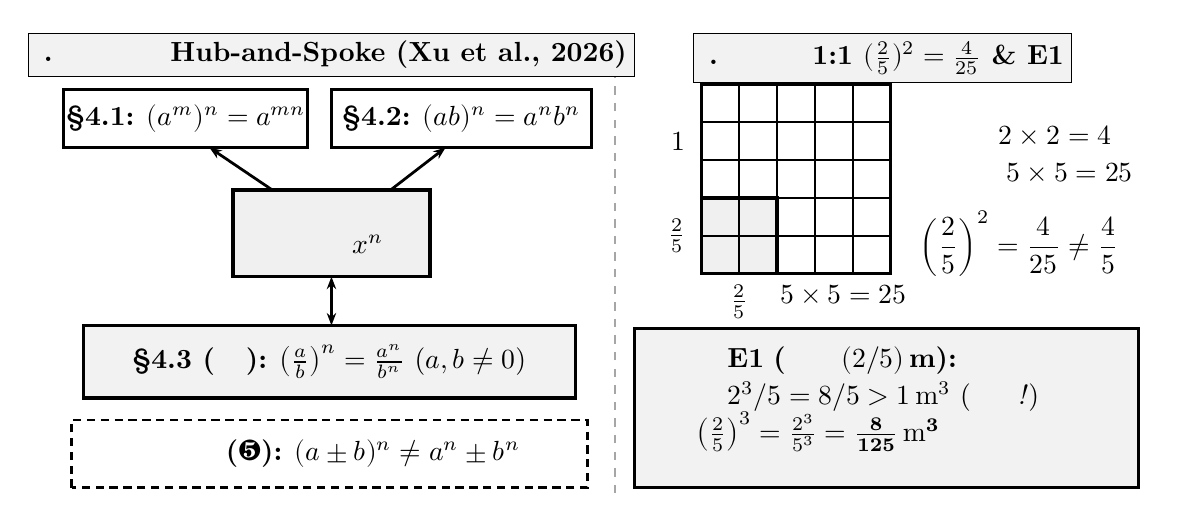
\begin{tikzpicture}[x=1cm, y=1cm, every node/.style={font=\linespread{1.0}\fontsize{10pt}{13.5pt}\selectfont, text=black}]
  \draw[line width=0.7pt, dashed, gray!70] (7.05, 0.05) -- (7.05, 5.95);
  \node[anchor=north, fill=headgray, draw=black, line width=0.5pt, inner sep=2.8pt] at (3.45, 5.90) {\textbf{ក. រចនាសម្ព័ន្ធ \en{Hub-and-Spoke} (\en{Xu et al., 2026})}};
  \node[anchor=north, fill=headgray, draw=black, line width=0.5pt, inner sep=2.8pt] at (10.45, 5.90) {\textbf{ខ. គំរូក្រឡា \en{1:1} $(\frac{2}{5})^2=\frac{4}{25}$ \& \en{E1}}};

  % Left Panel: Hub-and-Spoke (x = 0.05 .. 6.75)
  \begin{scope}[shift={(0.05, 0.06)}]
    \draw[black, line width=1.2pt, fill=panelgray] (2.15, 2.74) rectangle (4.65, 3.84);
    \node[align=center] at (3.40, 3.27) {\textbf{មជ្ឈមណ្ឌល}\\ \textbf{ស្វ័យគុណ $x^n$}};

    \draw[black, line width=1.0pt, fill=white] (0.00, 4.38) rectangle (3.10, 5.12);
    \node[align=center] at (1.55, 4.75) {\textbf{§4.1:} $(a^m)^n = a^{mn}$};

    \draw[black, line width=1.0pt, fill=white] (3.40, 4.38) rectangle (6.70, 5.12);
    \node[align=center] at (5.05, 4.75) {\textbf{§4.2:} $(ab)^n = a^n b^n$};

    \draw[black, line width=1.2pt, fill=headgray] (0.25, 1.20) rectangle (6.50, 2.12);
    \node[align=center] at (3.37, 1.66) {\textbf{§4.3 (ថ្មី):} $\left(\frac{a}{b}\right)^n = \frac{a^n}{b^n}$ ($a,b\neq 0$)};

    \draw[black, line width=1.0pt, -{Stealth[length=4.5pt]}] (2.65, 3.84) -- (1.85, 4.38);
    \draw[black, line width=1.0pt, -{Stealth[length=4.5pt]}] (4.15, 3.84) -- (4.85, 4.38);
    \draw[black, line width=1.1pt, {Stealth[length=4.5pt]}-{Stealth[length=4.5pt]}] (3.40, 2.74) -- (3.40, 2.12);

    \draw[black, densely dashed, line width=0.9pt, fill=white] (0.10, 0.06) rectangle (6.65, 0.92);
    \node[align=center] at (3.37, 0.49) {\textbf{ព្រំដែនហាម (\cnum{5}):} $(a\pm b)^n \neq a^n\pm b^n$};
  \end{scope}

  % Right Panel: 1:1 Grid Model + E1 (x = 7.20 .. 13.75)
  \begin{scope}[shift={(7.25, 0.06)}]
    \begin{scope}[shift={(0.90, 2.78)}]
      \fill[panelgray] (0,0) rectangle (0.96, 0.96);
      \draw[black, line width=1.1pt] (0,0) rectangle (2.40, 2.40);
      \foreach \k in {0.48, 0.96, 1.44, 1.92} {
        \draw[black, line width=0.65pt] (\k, 0) -- (\k, 2.40);
        \draw[black, line width=0.65pt] (0, \k) -- (2.40, \k);
      }
      \draw[black, line width=1.4pt] (0,0) rectangle (0.96, 0.96);
      \node[anchor=east] at (-0.08, 0.48) {$\frac{2}{5}$};
      \node[anchor=east] at (-0.08, 1.68) {$1$};
      \node[anchor=north] at (0.48, -0.02) {$\frac{2}{5}$};
      \node[anchor=north] at (1.80, -0.02) {$5\times 5 = 25$};
    \end{scope}

    \node[anchor=west, align=left] at (3.55, 4.30) {ក្រឡាឈូស៖ $2\times 2 = 4$\\ ក្រឡាសរុប៖ $5\times 5 = 25$};
    \node[anchor=west, align=left] at (3.55, 3.16) {$\left(\dfrac{2}{5}\right)^2 = \dfrac{4}{25} \neq \dfrac{4}{5}$};

    \draw[black, line width=0.95pt, fill=headgray] (0.05, 0.06) rectangle (6.45, 2.08);
    \node[anchor=north west, align=left, text width=6.15cm] at (0.20, 1.98) {%
      \textbf{បេសកកម្ម \en{E1} (ធុងគូប $(2/5)\unit{m}$):}\\
      អន្ទាក់៖ $2^3/5 = 8/5 > 1\unit{m}^3$ (\textit{មិនអាច!})\\
      ពិត៖ $\left(\frac{2}{5}\right)^3 = \frac{2^3}{5^3} = \mathbf{\frac{8}{125}\unit{m}^3}$};
  \end{scope}
\end{tikzpicture}\par
\vspace{1.5pt}
{\fontsize{10.5pt}{15pt}\selectfont\textbf{រូបទី ១៖} ស្ថាបត្យកម្មមជ្ឈមណ្ឌល–កាំ \en{Hub-and-Spoke} ភ្ជាប់លក្ខណៈទាំង ៣ និងគំរូក្រឡា \en{1:1} ដោះស្រាយអន្ទាក់បំភ្លេចភាគបែងក្នុង \en{E1--E3} \en{(Xu et al., 2026; Johanning, 2017; Ulusoy, 2019)}។}
\end{tcolorbox}

% --- រូបទី ២ ---
\Needspace{2.2cm}
\begin{tcolorbox}[enhanced, sharp corners, colback=white, colframe=black, boxrule=0.8pt, top=3.5pt, bottom=3.5pt, left=5pt, right=5pt, before skip=2pt, after skip=3pt]
\centering
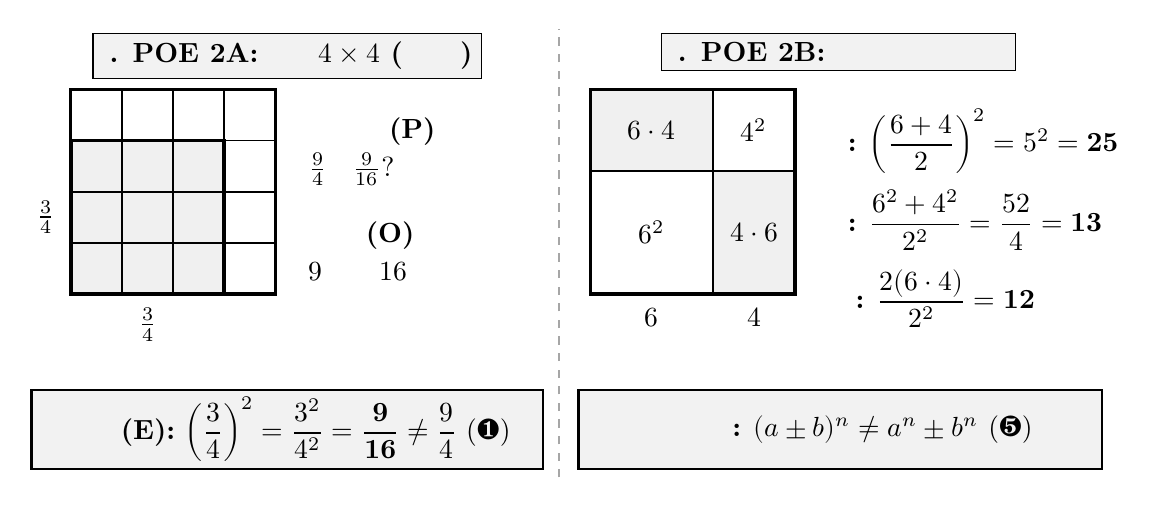
\begin{tikzpicture}[x=1cm, y=1cm, every node/.style={font=\linespread{1.0}\fontsize{10pt}{13.5pt}\selectfont, text=black}]
  \draw[line width=0.7pt, dashed, gray!70] (6.80, 0.05) -- (6.80, 5.75);
  \node[anchor=north, fill=headgray, draw=black, line width=0.5pt, inner sep=3.2pt] at (3.35, 5.70) {\textbf{ក. \en{POE 2A:} ក្រឡា $4\times 4$ \en{(}ទំព័រ ១\en{)}}};
  \node[anchor=north, fill=headgray, draw=black, line width=0.5pt, inner sep=3.2pt] at (10.35, 5.70) {\textbf{ខ. \en{POE 2B:} អន្ទាក់លីនេអ៊ែរលើផលបូក}};

  % Left Panel: POE 2A (4x4 with 3x3 shaded)
  \begin{scope}[shift={(0.05, 0.10)}]
    \begin{scope}[shift={(0.55, 2.28)}]
      \fill[panelgray] (0,0) rectangle (1.95, 1.95);
      \draw[black, line width=1.1pt] (0,0) rectangle (2.60, 2.60);
      \foreach \k in {0.65, 1.30, 1.95} {
        \draw[black, line width=0.65pt] (\k, 0) -- (\k, 2.60);
        \draw[black, line width=0.65pt] (0, \k) -- (2.60, \k);
      }
      \draw[black, line width=1.4pt] (0,0) rectangle (1.95, 1.95);
      \node[anchor=east] at (-0.08, 0.98) {$\frac{3}{4}$};
      \node[anchor=north] at (0.98, -0.05) {$\frac{3}{4}$};
    \end{scope}

    \node[anchor=west, align=left] at (3.45, 4.08) {\textbf{ទស្សន៍ទាយ \en{(P)}៖}\\ $\frac{9}{4}$ ឬ $\frac{9}{16}$?};
    \node[anchor=west, align=left] at (3.45, 2.82) {\textbf{សង្កេត \en{(O)}៖}\\ $9$ ក្នុង $16$ ក្រឡា};

    \draw[black, line width=0.9pt, fill=headgray] (0.05, 0.06) rectangle (6.55, 1.06);
    \node[align=center] at (3.30, 0.56) {\textbf{ពន្យល់ \en{(E)}:} $\left(\dfrac{3}{4}\right)^2 = \dfrac{3^2}{4^2} = \mathbf{\dfrac{9}{16}} \neq \dfrac{9}{4}$ (\cnum{1})};
  \end{scope}

  % Right Panel: POE 2B ((6+4)/2)^2 vs (6^2+4^2)/2^2
  \begin{scope}[shift={(7.00, 0.10)}]
    \begin{scope}[shift={(0.20, 2.28)}]
      \fill[panelgray] (0, 1.56) rectangle (1.56, 2.60);
      \fill[panelgray] (1.56, 0) rectangle (2.60, 1.56);
      \draw[black, line width=1.15pt] (0,0) rectangle (2.60, 2.60);
      \draw[black, line width=0.9pt] (1.56, 0) -- (1.56, 2.60);
      \draw[black, line width=0.9pt] (0, 1.56) -- (2.60, 1.56);
      \node at (0.78, 0.78) {$6^2$};
      \node at (2.08, 2.08) {$4^2$};
      \node at (0.78, 2.08) {$6\cdot 4$};
      \node at (2.08, 0.78) {$4\cdot 6$};
      \node[anchor=north] at (0.78, -0.05) {$6$};
      \node[anchor=north] at (2.08, -0.05) {$4$};
    \end{scope}

    \node[anchor=west, align=left] at (3.05, 4.22) {\textbf{ពិត:} $\left(\dfrac{6+4}{2}\right)^2 = 5^2 = \mathbf{25}$};
    \node[anchor=west, align=left] at (3.05, 3.22) {\textbf{ខុស:} $\dfrac{6^2+4^2}{2^2} = \dfrac{52}{4} = \mathbf{13}$};
    \node[anchor=west, align=left] at (3.05, 2.22) {\textbf{បាត់:} $\dfrac{2(6\cdot 4)}{2^2} = \mathbf{12}$};

    \draw[black, line width=0.9pt, fill=headgray] (0.05, 0.06) rectangle (6.70, 1.06);
    \node[align=center] at (3.37, 0.56) {\textbf{ហាមលីនេអ៊ែរ:} $(a\pm b)^n \neq a^n\pm b^n$ (\cnum{5})};
  \end{scope}
\end{tikzpicture}\par
\vspace{2pt}
{\fontsize{10.5pt}{15pt}\selectfont\textbf{រូបទី ២៖} ពិសោធន៍ \en{Dual POE 2A--2B} ផ្គូផ្គងច្បាប់ចែកចាយផលចែកត្រឹមត្រូវទន្ទឹមនឹងឧទាហរណ៍ជំទាស់លើផលបូក \en{(Rolfes et al., 2020; Van Dooren et al., 2003; Fitria et al., 2023)}។}
\end{tcolorbox}

% --- រូបទី ៣ ---
\Needspace{2.2cm}
\begin{tcolorbox}[enhanced, sharp corners, colback=white, colframe=black, boxrule=0.8pt, top=3.5pt, bottom=3.5pt, left=5pt, right=5pt, before skip=2pt, after skip=3pt]
\centering
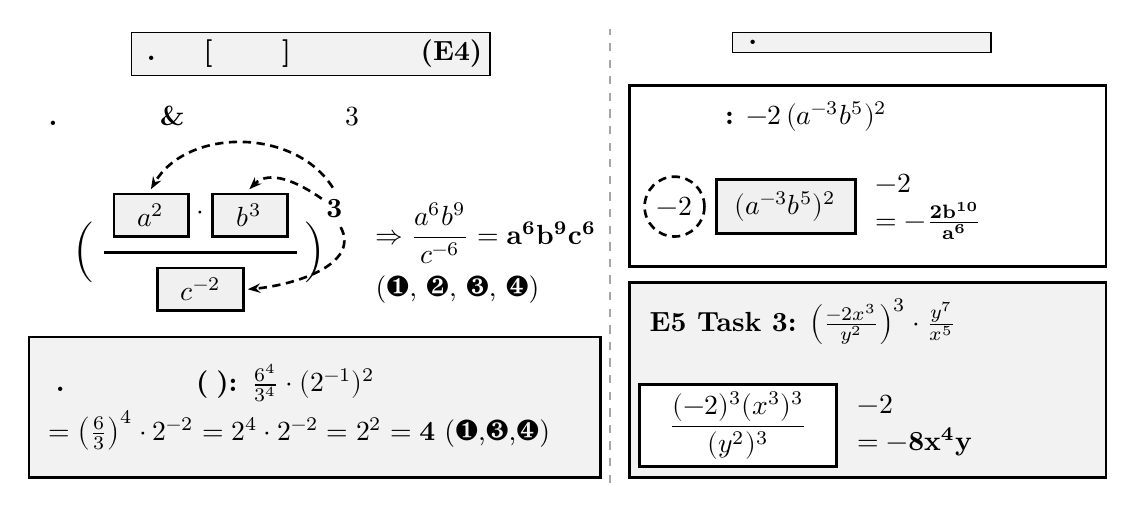
\begin{tikzpicture}[x=1cm, y=1cm, every node/.style={font=\linespread{1.0}\fontsize{10pt}{13.5pt}\selectfont, text=black}]
  \draw[line width=0.7pt, dashed, gray!70] (7.45, 0.05) -- (7.45, 5.82);
  \node[anchor=north, fill=headgray, draw=black, line width=0.5pt, inner sep=2.8pt] at (3.65, 5.78) {\textbf{ក. អូស [ចង្អុលអូស] ពីក្រៅចូលក្នុង \en{(E4)}}};
  \node[anchor=north, fill=headgray, draw=black, line width=0.5pt, inner sep=2.8pt] at (10.65, 5.78) {\textbf{ខ. វិសាលភាពសញ្ញាដក និងវង់ក្រចក}};

  % Left Panel: Outside-In Tracing on ((a^2 b^3)/c^-2)^3 & Reverse Consolidation
  \begin{scope}[shift={(0.05, 0.06)}]
    \node[anchor=west] at (0.05, 4.65) {\textbf{១. ព័ទ្ធកត្តា \& អូសពីនិទស្សន្តក្រៅ $3$៖}};
    \draw[black, line width=1.0pt, fill=panelgray] (1.10, 3.12) rectangle (2.05, 3.66);
    \node at (1.57, 3.39) {$a^2$};
    \node at (2.20, 3.39) {$\cdot$};
    \draw[black, line width=1.0pt, fill=panelgray] (2.35, 3.12) rectangle (3.30, 3.66);
    \node at (2.82, 3.39) {$b^3$};
    \draw[black, line width=1.1pt] (0.98, 2.92) -- (3.42, 2.92);
    \draw[black, line width=1.0pt, fill=panelgray] (1.65, 2.18) rectangle (2.75, 2.72);
    \node at (2.20, 2.45) {$c^{-2}$};
    \node at (0.72, 2.92) {\fontsize{22pt}{22pt}\selectfont(};
    \node[at={(3.64, 2.92)}] {\fontsize{22pt}{22pt}\selectfont)};
    \node[inner sep=2pt] (exp3) at (3.90, 3.48) {\textbf{3}};

    % Tracing dashed arrows from outer 3 (all origins clearly outside the '3' glyph)
    \draw[black, densely dashed, line width=0.95pt, -{Stealth[length=4.5pt]}] (3.88, 3.74) to[out=122, in=60] (1.57, 3.72);
    \draw[black, densely dashed, line width=0.95pt, -{Stealth[length=4.5pt]}] (3.74, 3.60) to[out=145, in=45] (2.82, 3.72);
    \draw[black, densely dashed, line width=0.95pt, -{Stealth[length=4.5pt]}] (3.98, 3.24) to[out=-62, in=5] (2.80, 2.45);

    \node[anchor=west] at (4.30, 3.16) {$\Rightarrow \dfrac{a^6 b^9}{c^{-6}} = \mathbf{a^6 b^9 c^6}$};
    \node[anchor=west] at (4.30, 2.44) {(\cnum{1}, \cnum{2}, \cnum{3}, \cnum{4})};

    \draw[black, line width=0.85pt, fill=headgray] (0.02, 0.06) rectangle (7.28, 1.84);
    \node[anchor=west, align=left, text width=7.02cm] at (0.14, 0.95) {%
      \textbf{២. ទិសច្រាសពង្រឹង (គ):} $\frac{6^4}{3^4}\cdot(2^{-1})^2$\\[2pt]
      $= \left(\frac{6}{3}\right)^4\cdot 2^{-2} = 2^4\cdot 2^{-2} = 2^2 = \mathbf{4}$ (\cnum{1},\cnum{3},\cnum{4})};
  \end{scope}

  % Right Panel: Sign scope contrast
  \begin{scope}[shift={(7.65, 0.06)}]
    \draw[black, line width=0.9pt, fill=white] (0.05, 2.74) rectangle (6.10, 5.04);
    \node[anchor=north west] at (0.18, 4.96) {\textbf{ជំហាន ២ ក:} $-2\,(a^{-3}b^5)^2$};
    \draw[black, line width=0.95pt, densely dashed] (0.62, 3.50) circle (0.38cm);
    \node at (0.62, 3.50) {$-2$};
    \draw[black, line width=1.05pt, fill=panelgray] (1.15, 3.16) rectangle (2.92, 3.84);
    \node at (2.03, 3.50) {$(a^{-3}b^5)^2$};
    \node[anchor=west, align=left] at (3.05, 3.50) {$-2$ \textbf{នៅក្រៅ}\\ $= \mathbf{-\frac{2b^{10}}{a^6}}$};

    \draw[black, line width=1.05pt, fill=headgray] (0.05, 0.06) rectangle (6.10, 2.54);
    \node[anchor=north west] at (0.18, 2.46) {\textbf{\en{E5 Task 3:}} $\left(\frac{-2x^3}{y^2}\right)^3\cdot\frac{y^7}{x^5}$};
    \draw[black, line width=1.1pt, fill=white] (0.18, 0.20) rectangle (2.68, 1.24);
    \node at (1.43, 0.72) {$\dfrac{(-2)^3(x^3)^3}{(y^2)^3}$};
    \node[anchor=west, align=left] at (2.82, 0.72) {$-2$ \textbf{នៅក្នុង}\\ $= \mathbf{-8x^4 y}$};
  \end{scope}
\end{tikzpicture}\par
\vspace{1.5pt}
{\fontsize{10.5pt}{15pt}\selectfont\textbf{រូបទី ៣៖} លំហូរអូសម្រាមដៃ [ចង្អុលអូស] ពីនិទស្សន្តក្រៅទៅភាគយកនិងភាគបែង (\en{E4}) និងការញែកវិសាលភាពសញ្ញាដកក្រៅ/ក្នុងវង់ក្រចក \en{(Yeo \& Tzeng, 2019; Olson et al., 2011; Rohrer et al., 2020)}។}
\end{tcolorbox}

% --- រូបទី ៤ ---
\Needspace{2.2cm}
\begin{tcolorbox}[enhanced, sharp corners, colback=white, colframe=black, boxrule=0.8pt, top=3.5pt, bottom=3.5pt, left=5pt, right=5pt, before skip=2pt, after skip=3pt]
\centering
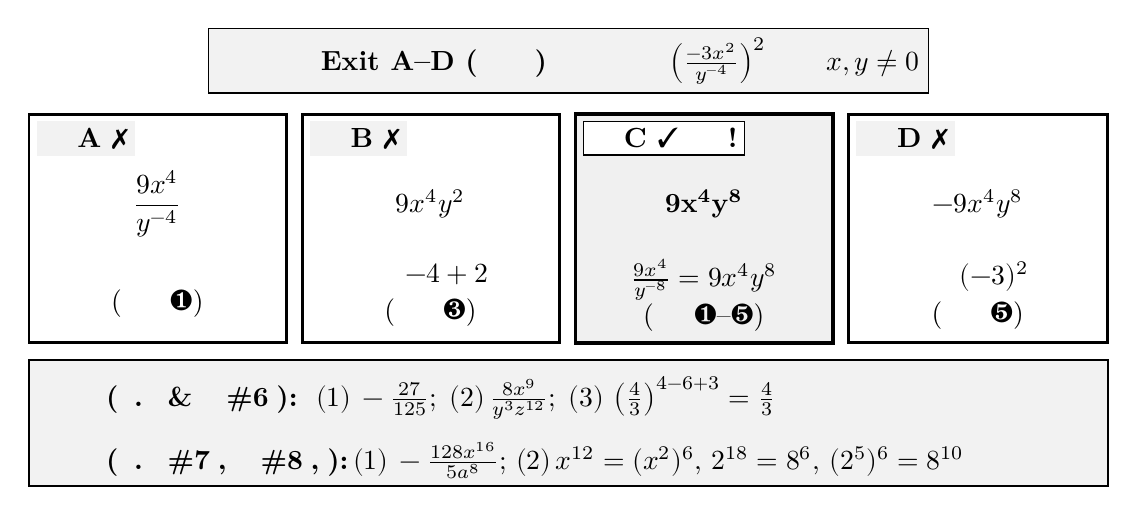
\begin{tikzpicture}[x=1cm, y=1cm, every node/.style={font=\linespread{1.0}\fontsize{10pt}{13.5pt}\selectfont, text=black}]
  \node[anchor=north, fill=headgray, draw=black, line width=0.6pt, inner sep=3.2pt] at (6.90, 5.88) {\textbf{កាតវិនិច្ឆ័យ \en{Exit A--D} (ទំព័រ ៥)៖ សម្រួលកន្សោម $\left(\frac{-3x^2}{y^{-4}}\right)^2$ ចំពោះ $x, y \neq 0$}};

  \draw[black, line width=0.95pt] (0.05, 1.88) rectangle (3.32, 4.78);
  \node[anchor=north west, fill=headgray, inner sep=2.5pt] at (0.14, 4.70) {\textbf{កាត \en{A} \ding{55}}};
  \node[align=center] at (1.68, 3.64) {$\dfrac{9x^4}{y^{-4}}$};
  \node[align=center] at (1.68, 2.48) {ភ្លេចភាគបែង\\ (\textit{ល្មើស} \cnum{1})};

  \draw[black, line width=0.95pt] (3.52, 1.88) rectangle (6.79, 4.78);
  \node[anchor=north west, fill=headgray, inner sep=2.5pt] at (3.61, 4.70) {\textbf{កាត \en{B} \ding{55}}};
  \node[align=center] at (5.15, 3.64) {$9x^4 y^2$};
  \node[align=center] at (5.15, 2.48) {បូក $-4+2$\\ (\textit{ល្មើស} \cnum{3})};

  \draw[black, line width=1.35pt, fill=panelgray] (6.99, 1.88) rectangle (10.26, 4.78);
  \node[anchor=north west, fill=white, draw=black, line width=0.5pt, inner sep=2.5pt] at (7.08, 4.70) {\textbf{កាត \en{C} \ding{51} ត្រូវ!}};
  \node[align=center] at (8.62, 3.64) {$\mathbf{9x^4 y^8}$};
  \node[align=center] at (8.62, 2.48) {$\frac{9x^4}{y^{-8}}=9x^4y^8$\\ (\textit{ប្រើ} \cnum{1}--\cnum{5})};

  \draw[black, line width=0.95pt] (10.46, 1.88) rectangle (13.75, 4.78);
  \node[anchor=north west, fill=headgray, inner sep=2.5pt] at (10.55, 4.70) {\textbf{កាត \en{D} \ding{55}}};
  \node[align=center] at (12.10, 3.64) {$-9x^4 y^8$};
  \node[align=center] at (12.10, 2.48) {ខុស $(-3)^2$\\ (\textit{ល្មើស} \cnum{5})};

  \draw[black, line width=0.85pt, fill=headgray] (0.05, 0.06) rectangle (13.75, 1.66);
  \node[anchor=north west, text width=13.45cm] at (0.18, 1.58) {\textbf{ផ្ទះ ក (ទំ.១៨ \& ២៥ \en{\#6}គ):}\, $(1)\,-\frac{27}{125};\; (2)\,\frac{8x^9}{y^3z^{12}};\; (3)\,\left(\frac{4}{3}\right)^{4-6+3}=\frac{4}{3}$};
  \node[anchor=north west, text width=13.45cm] at (0.18, 0.74) {\textbf{ផ្ទះ ខ (ទំ.២៥ \en{\#7}ង, ២៦ \en{\#8}ក,គ):}\,$(1)\,-\frac{128x^{16}}{5a^8};\, (2)\,x^{12}=(x^2)^6,\,2^{18}=8^6,\,(2^5)^6=8^{10}$};
\end{tikzpicture}\par
\vspace{1.5pt}
{\fontsize{10.5pt}{15pt}\selectfont\textbf{រូបទី ៤៖} កាតត្រួតពិនិត្យរហ័ស \en{Exit A--D} (ទំព័រ ៥) ចាប់កំហុសទាំង ៤ និងសោចម្លើយកិច្ចការផ្ទះទំព័រ ១៨, ២៥--២៦ \en{(Ulusoy, 2019; Olson et al., 2011; Rohrer et al., 2020)}។}
\end{tcolorbox}

% ============================================================================
% ផ្នែកទី ៤៖ សេណារីយ៉ូពាក្យពេចន៍គ្រូបង្រៀនផ្ទាល់ និងការគ្រប់គ្រងក្ដារខៀន
% ============================================================================
\secbanner{ផ្នែកទី ៤៖ សេណារីយ៉ូពាក្យពេចន៍គ្រូបង្រៀនផ្ទាល់ និងការគ្រប់គ្រងក្ដារខៀន}{Section 4: Verbatim Teacher Scripts (00--50 min), Pause-Ask/Review Gates \& 3-Zone Blackboard Plan}

ពាក្យពេចន៍គ្រូបង្រៀនផ្ទាល់ខាងក្រោមត្រូវបានរៀបចំតាមដំណាក់កាលនីមួយៗឱ្យស៊ីចង្វាក់ \en{100\%} ជាមួយ \en{LS\_Plan\_\allowbreak POWQ} និង \en{Teaching\_\allowbreak Scenario\_\allowbreak POWQ}។

\Needspace{2.0cm}
\begin{phasebox}{ជំហាន ១ \enbf{\&} ២ក\enbf{--}ខ៖ រដ្ឋបាល កំណែប្រតិបត្តិ ៤\enbf{.}២ និងរំលឹក}{00--08 min}{8 នាទី}
\textbf{គោលបំណង}៖ រៀបចំក្រុម ៣ នាក់, កែកិច្ចការផ្ទះប្រតិបត្តិ \en{4.2} (ទំ.១៨) ផ្ទៀងវិសាលភាព $-2$ និងពុម្ពទំ.១៧ \en{vs} ១៨, រួចរំលឹក \en{§3, §4.1, §4.2} \en{(Olson et al., 2011; Wang et al., 2026)}។
\end{phasebox}
\begin{scriptbox}
  \textbf{នាទី \en{00--02} (រដ្ឋបាល) — }\teachersays{សួស្ដីប្អូនៗ! ថ្ងៃនេះក្រុម ៣ នាក់របស់យើងបែងចែកតួនាទី ៣ គឺ៖ តួនាទី ១ (អ្នកគូស [ចង្អុលអូស] និងពិនិត្យសញ្ញា \en{B\&W}), តួនាទី ២ (អ្នកភ្ជាប់ហេតុផល \cnum{1}--\cnum{5} និងគណនា), តួនាទី ៣ (អ្នកត្រួតពិនិត្យលក្ខខណ្ឌ $a,b\neq 0$ និងសញ្ញាដក)។ សូមរៀបកន្ត្រៃ និងបន្ទាត់ \en{cm} លើតុ ហើយទុកក្រដាសទំព័រ ១ ផ្កាប់ចុះក្រោមសិន — កុំទាន់កាត់មុនបញ្ជាគ្រូ!}\par\vspace{3pt}
  \textbf{នាទី \en{02--05} (កំណែប្រតិបត្តិ ៤.២ $\le 3'$) — }\teachersays{ផ្ទៀងកំណែ \textbf{ប្រតិបត្តិ ៤.២ (ទំ.១៨)}៖ \textbf{ក.} $-2(a^{-3}\cdot b^5)^2 = -2(a^{-6}\cdot b^{10}) = -2a^{-6}b^{10} = -\frac{2b^{10}}{a^6}$ ($a\neq 0$)។ សួរថា៖ ហេតុអ្វី $-2$ មិនក្លាយជា $+4$?}\par\vspace{2pt}
  \textbf{$\circ$ សិស្ស៖} \textit{«ព្រោះ $-2$ នៅក្រៅវង់ក្រចក មិនជាប់និទស្សន្ត $2$ ទេលោកគ្រូ!»}\par\vspace{2pt}
  \teachersays{ត្រឹមត្រូវ! ចំណែក \textbf{ខ.} $a\cdot(a^4)^5\cdot a^{-6} = a^1\cdot a^{20}\cdot a^{-6} = a^{1+20-6} = a^{15}$ ($a\neq 0$)។ ប្រយ័ត្ន! នៅទំ.១៧ សៀវភៅបោះពុម្ព $(a^4)^5$ បាន $a^{15}$ រីឯនៅទំ.១៨ បោះពុម្ពបាត់និទស្សន្តក្រៅ $5$ ក្លាយជា $a\cdot(a^4)\cdot a^{-6} = a^{-1} = \frac{1}{a}$ — ត្រូវអានវង់ក្រចកជាក់ស្ដែងជានិច្ច!}\par\vspace{3pt}
  \textbf{នាទី \en{05--08} (រំលឹក ៣') — }\teachersays{រំលឹករហ័ស ៣ វិធាន៖ \textbf{§3} $\frac{a^m}{a^n} = a^{m-n},\; a^0 = 1,\; a^{-n} = \frac{1}{a^n}$ ($a\neq 0$); \textbf{§4.1} $(a^m)^n = a^{mn}$; និង \textbf{§4.2} $(ab)^n = a^n b^n$។ តើ $\frac{1}{c^{-2}}$ ស្មើប៉ុន្មាន?}\par\vspace{2pt}
  \textbf{$\circ$ សិស្ស៖} \textit{«ស្មើ $c^2$ ព្រោះភាគបែងមាននិទស្សន្តដកប្ដូរឡើងទៅលើវិញ!»}
\end{scriptbox}

\Needspace{2.0cm}
\begin{phasebox}{ជំហាន ២គ \enbf{(E1 - Engage)}៖ បេសកកម្មធុងស្តុកទឹក និងសំណាញ់ព្រះក្រសាំង}{08--11 min}{3 នាទី}
\textbf{គោលបំណង}៖ ដាស់ទស្សន៍ទាយ និងលាតត្រដាងអន្ទាក់បំភ្លេចភាគបែង $\frac{2^3}{5}=\frac{8}{5}>1\unit{m}^3$ \en{(Leton et al., 2026; Johanning, 2017)}។
\end{phasebox}
\begin{scriptbox}
  \textbf{នាទី \en{08--11} — }\teachersays{សូមស្វាគមន៍មកកាន់ \textbf{«បេសកកម្មកាត់បង្រួមធុងស្តុកទឹក និងផ្ទាំងសំណាញ់នៅព្រះក្រសាំង»}! ធុងគូបដើមមានជ្រុង $1\unit{m}$ ផ្ទុកទឹក $1\unit{m}^3$។ ជាងសំណង់បង្រួមជ្រុងធុងមកត្រឹម $\frac{2}{5}\unit{m}$ រួចសិស្សម្នាក់គណនាមាឌថ្មីថា $\left(\frac{2}{5}\right)^3 = \frac{2^3}{5} = \frac{8}{5}\unit{m}^3$! តើធុងកាត់បង្រួមតូចជាងមុន អាចផ្ទុកទឹកបានដល់ $\frac{8}{5}=1.6\unit{m}^3$ ធំជាងធុងដើម $1\unit{m}^3$ ដែរឬទេ? ហេតុអ្វី?}\par\vspace{2pt}
  \textbf{$\circ$ សកម្មភាពសិស្ស៖} ក្រុមពិភាក្សាទស្សន៍ទាយ (\textit{«មិនអាចទេលោកគ្រូ! ព្រោះជ្រុងខ្លីជាង $1\unit{m}$!»})។ គ្រូកត់ទស្សន៍ទាយលើក្ដារខៀន \textbf{ដោយទុកចម្លើយចុងក្រោយសម្រាប់បិទបញ្ចប់នៅ \en{E5}}។
\end{scriptbox}

\Needspace{2.0cm}
\begin{phasebox}{ជំហាន ៣ក \enbf{(E2 - Explore)}៖ ពិសោធន៍ក្រឡា ១\enbf{:}១ និង \enbf{Dual POE 2A--2B}}{11--22 min}{11 នាទី}
\textbf{គោលបំណង}៖ រកឃើញ $\left(\frac{a}{b}\right)^n = \frac{a^n}{b^n}$ តាមក្រឡា \en{1:1} និងកត្តាទំ.១៨, រួចទាត់ចោលអន្ទាក់លីនេអ៊ែរលើផលបូក \en{(Johanning, 2017; Rolfes et al., 2020; Van Dooren et al., 2003)}។
\end{phasebox}
\begin{scriptbox}
  \textbf{នាទី \en{11--17} (ស.១ ក្រឡា \en{1:1}, ទំព័រ ១) — }\teachersays{ត្រឡប់ទំព័រ ១ ឡើង! ដំបូង យកបន្ទាត់វាស់ \textbf{បន្ទាត់ក្រិត \en{5.00 cm}} ខាងលើឱ្យច្បាស់ថាព្រីនខ្នាត \en{1:1 Actual Size 100\%}។ កាត់បន្ទះឈូស $2.00\times 2.00\unit{cm}$ ដាក់លើក្រឡាឯកតា $5.00\times 5.00\unit{cm}$ ដែលមាន $25$ ការ៉េ។ តើបន្ទះឈូសគ្របដណ្ដប់ប៉ុន្មានការ៉េក្នុង $25$ ការ៉េ?}\par\vspace{2pt}
  \textbf{$\circ$ សិស្ស៖} \textit{«គ្រប $4$ ការ៉េក្នុង $25$ ការ៉េ! ដូច្នេះ $\left(\frac{2}{5}\right)^2 = \frac{4}{25} \neq \frac{4}{5}$ ($0.16 < 0.40$ មិនមែន $0.80$ ទេ)!»}\par\vspace{2pt}
  \teachersays{ប្រសើរណាស់! តួនាទី ៣ សូមផ្ទៀងជាមួយក្រុមថា ហេតុអ្វីទំហំតូចជាង $\frac{2}{5}$? ព្រោះ $\frac{2}{5}<1$ កាលណាលើកស្វ័យគុណ ២ ទំហំផ្ទៃកាន់តែតូច។ ឥឡូវផ្គុំកត្តាតាម \textbf{ឧទាហរណ៍ ទំ.១៨}៖ \textbf{ក.} $\frac{2^3}{5^3} = \frac{2\times 2\times 2}{5\times 5\times 5} = \left(\frac{2}{5}\right)\left(\frac{2}{5}\right)\left(\frac{2}{5}\right) = \left(\frac{2}{5}\right)^3$ និង \textbf{ខ.} $\frac{a^n}{b^n} = \frac{a\cdot a\cdots a}{b\cdot b\cdots b} = \left(\frac{a}{b}\right)^n$។}\par\vspace{3pt}
  \textbf{នាទី \en{17--22} (ស.២ \en{Dual POE 2A--2B}, ទំព័រ ១) — }\teachersays{ចូល \textbf{\en{POE 2A}}៖ មើលក្រឡា $4.00\times 4.00\unit{cm}$ និងការ៉េឈូស $3.00\times 3.00\unit{cm}$ — គូសប្រអប់ \textbf{ទស្សន៍ទាយ (\en{P})} រួចរាប់ផ្ទៀង \textbf{(\en{O})}! តើ $\left(\frac{3}{4}\right)^2$ ស្មើប៉ុន្មាន?}\par\vspace{2pt}
  \textbf{$\circ$ សិស្ស៖} \textit{«បាន $9$ ក្នុង $16$ ការ៉េ $\Rightarrow \left(\frac{3}{4}\right)^2 = \frac{9}{16} \neq \frac{9}{4}$ ($\frac{9}{16}<1$ ខណៈ $\frac{9}{4}=2.25>1$)!»}\par\vspace{2pt}
  \teachersays{ឥឡូវសាក \textbf{\en{POE 2B} (ឧទាហរណ៍ជំទាស់)}៖ គណនា $\left(\frac{6+4}{2}\right)^2$ ធៀបនឹង $\frac{6^2+4^2}{2^2}$! តើស្មើគ្នាទេ?}\par\vspace{2pt}
  \textbf{$\circ$ សិស្ស៖} \textit{«ទេលោកគ្រូ! ខាងឆ្វេងបាន $5^2=25$ ឯខាងស្ដាំបាន $\frac{36+16}{4}=\frac{52}{4}=13$ — ស្វ័យគុណ\textbf{មិនចែកចាយលើផលបូក $+$} ទេ!»}\par\vspace{2pt}
  \teachersays{ចងចាំច្បាប់មាសនេះឱ្យច្បាស់៖ ស្វ័យគុណចែកចាយលើ\textbf{ផលចែក} ($\div$) បានត្រឹមត្រូវ ប៉ុន្តែ\textbf{ហាម}ចែកចាយលើផលបូក ($+$) ឬផលដក ($-$) ជាដាច់ខាត!}
\end{scriptbox}

\Needspace{2.0cm}
\begin{phasebox}{ជំហាន ៣ខ \enbf{(E3 - Explain)}៖ បង្គុំទ្រឹស្ដី ៤\enbf{.}៣ \enbf{Hub-and-Spoke} និងធនាគារ \cnum{1}\enbf{--}\cnum{5}}{22--28 min}{6 នាទី}
\textbf{គោលបំណង}៖ សិស្សបង្គុំប្រអប់ «ជាទូទៅ ៤.៣» (ពីរទិស និងច្បាប់ច្រាសដក), ដ្យាក្រាម $x^n$ និងផ្ទាំង \cnum{1}--\cnum{5} \en{(Xu et al., 2026; Vest et al., 2022)}។
\end{phasebox}
\begin{scriptbox}
  \textbf{នាទី \en{22--28} (ទំព័រ ៤) — }\teachersays{សូមសិស្សបំពេញប្រអប់ \textbf{«ជាទូទៅ ៤.៣» (ទំ.១៨)}៖ បើ $a, b$ ជាចំនួនសនិទានខុសពីសូន្យ និង $n$ ជាចំនួនគត់រ៉ឺឡាទីបខុសពីសូន្យ គេបាន $\left(\frac{a}{b}\right)^n = \frac{a^n}{b^n}$។ ចុះបើអានពីស្ដាំទៅឆ្វេង និងពេលនិទស្សន្តដក $\left(\frac{a}{b}\right)^{-n}$ តើយើងបានអ្វី?}\par\vspace{2pt}
  \textbf{$\circ$ សិស្ស៖} \textit{«ទិសច្រាស $\frac{a^n}{b^n} = \left(\frac{a}{b}\right)^n$ និងពេលដក $\left(\frac{a}{b}\right)^{-n} = \frac{a^{-n}}{b^{-n}} = \frac{b^n}{a^n} = \left(\frac{b}{a}\right)^n$!»}\par\vspace{2pt}
  \teachersays{ប្រសើរណាស់! មើលផែនទី \textbf{\en{Hub-and-Spoke}} ជុំវិញ $x^n$៖ កាំទី ១ $(a^m)^n=a^{mn}$ (\cnum{3}), កាំទី ២ $(ab)^n=a^nb^n$ (\cnum{2}), កាំទី ៣ $\left(\frac{a}{b}\right)^n=\frac{a^n}{b^n}$ (\cnum{1})។ ចងចាំព្រំដែន $(a\pm b)^n\neq a^n\pm b^n$ (\cnum{5})! គ្រូបិទ \textbf{ផ្ទាំងធនាគារហេតុផល \cnum{1}--\cnum{5} (ទំព័រ ៤)} នៅកណ្ដាលក្ដារខៀន!}
\end{scriptbox}

\Needspace{2.0cm}
\begin{phasebox}{ជំហាន ៤ក \enbf{(E4 - Elaborate)}៖ កាត \enbf{B\&W [}ចង្អុលអូស\enbf{]} និង \enbf{EIA Looking-Back}}{28--38 min}{10 នាទី}
\textbf{គោលបំណង}៖ ហ្វឹកហាត់លំហាត់គំរូទី ១ (ទំ.១៨ ក, ខ) និងពង្រឹងទិសច្រាស គ ដោយ [ចង្អុលអូស] និង \en{EIA 30s} \en{(Yeo \& Tzeng, 2019; Rohrer et al., 2020; Runisah et al., 2017)}។
\end{phasebox}
\begin{scriptbox}
  \textbf{នាទី \en{28--38} (ទំព័រ ២) — }\teachersays{ចែកកាត \en{E4} (ទំព័រ ២)! អនុវត្ត ៣ ជំហាន៖ ១) អូស [ចង្អុលអូស] ពីនិទស្សន្តក្រៅទៅភាគយកនិងភាគបែង, ២) ចុះលេខ \cnum{1}--\cnum{5} គណនា, ៣) \en{EIA Looking-Back}។ មើល \textbf{ក.} $\left(\frac{3}{4}\right)^3 = \frac{3^3}{4^3} = \frac{27}{64}$ (\cnum{1})។ មើល \textbf{ខ.} $\left(\frac{a^2b^3}{c^{-2}}\right)^3$ — អូសនិទស្សន្ត $3$ ចូលទាំង $a^2$, $b^3$ និង $c^{-2}$៖ $\frac{(a^2)^3(b^3)^3}{(c^{-2})^3} = \frac{a^6b^9}{c^{-6}} = a^6b^9c^6$ ($c\neq 0$, \cnum{1}, \cnum{2}, \cnum{3}, \cnum{4})! មើល \textbf{គ. (ទិសច្រាសពង្រឹង)}៖ $\frac{6^4}{3^4}\cdot(2^{-1})^2 = \left(\frac{6}{3}\right)^4\cdot 2^{-2} = 2^4\cdot 2^{-2} = 2^2 = 4$ (\cnum{1} ច្រាស, \cnum{3}, \cnum{4})!}\par\vspace{2pt}
  \teachersays{\textbf{សំណួរ \en{EIA Looking-Back (30s)}:} ១) ហេតុអ្វី $c^{-6}$ នៅភាគបែងក្លាយជា $c^6$ នៅភាគយក? ២) បើមិនប្ដូរ $\frac{6^4}{3^4}$ ទៅ $\left(\frac{6}{3}\right)^4$ តើពិបាកគណនា $6^4$ យ៉ាងណា?}\par\vspace{2pt}
  \textbf{$\circ$ សិស្ស៖} \textit{«១) តាម $\frac{1}{c^{-n}}=c^n$ (\cnum{4}); ២) $6^4=1\,296$ ចែក $81$ យូរ ឯផ្គុំជា $2^4=16$ គុណ $2^{-2}$ បាន $4$ ភ្លាម!»}
\end{scriptbox}

\Needspace{2.0cm}
\begin{phasebox}{ជំហាន ៤ខ \enbf{(E5)} \& ៥៖ \enbf{Relay} ៣ តួនាទី\enbf{,} កាត \enbf{A--D} និងកិច្ចការផ្ទះ}{38--50 min}{12 នាទី}
\textbf{គោលបំណង}៖ វាយតម្លៃ \en{Relay} ៣ តួនាទី (\en{Pause-Ask / Pause-Review}), បិទបេសកកម្ម \en{E1}, កាត \en{Exit A--D} + \en{Exit Ticket} និងចែកកិច្ចការផ្ទះ \en{(Wang et al., 2026; Kshetree et al., 2021; Rohrer et al., 2020)}។
\end{phasebox}
\begin{scriptbox}
  \textbf{នាទី \en{38--44.5} (\en{Relay 3} តួនាទី, ទំព័រ ៣) — }\teachersays{ចែកសន្លឹក \en{Relay} ទំព័រ ៣! ក្រុមធ្វើ \textbf{Task 1} (ប្រតិបត្តិ ក): $\left(\frac{-2}{3}\right)^4$, \textbf{Task 2} (ប្រតិបត្តិ ខ): $\left(\frac{a^4\cdot b^{-2}}{c^3}\right)^2$, និង \textbf{Task 3} (សំយោគ ៣ លក្ខណៈ): $\left(\frac{-2x^3}{y^2}\right)^3\cdot\frac{y^7}{x^5}$! \textbf{តួនាទី ១ (\en{Pause-Ask!})៖} គូស [ចង្អុលអូស] និងសួរដៃគូ៖ \textit{«តើ $(-2)^4$ វិជ្ជមានឬអវិជ្ជមាន? ចុះ $(-2)^3$?»} \textbf{តួនាទី ២} គណនានិងចុះលេខ \cnum{1}--\cnum{5}៖ Task 1 $=\frac{16}{81}$, Task 2 $=\frac{a^8b^{-4}}{c^6}=\frac{a^8}{b^4c^6}$ ($b,c\neq 0$), Task 3 $=\frac{-8x^9}{y^6}\cdot\frac{y^7}{x^5}=-8x^4y$ ($x,y\neq 0$)។ \textbf{តួនាទី ៣ (\en{Pause-Review!})៖} ផ្ទៀងសញ្ញាដក កុំភ្លេច $2^3=8$ និងលក្ខខណ្ឌ $x,y\neq 0$! \textbf{បិទបេសកកម្ម \en{E1}៖} ឥឡូវធុងគូបជ្រុង $\frac{2}{5}\unit{m}$ ផ្ទុកទឹកបានប៉ុន្មាន? ($\left(\frac{2}{5}\right)^3 = \frac{2^3}{5^3} = \frac{8}{125}\unit{m}^3 < 1\unit{m}^3$!)}\par\vspace{3pt}
  \textbf{នាទី \en{44.5--48} (កាត \en{Exit A--D} \& សំបុត្រចេញ ទំព័រ ៥) — }\teachersays{មើលកន្សោម $\left(\frac{-3x^2}{y^{-4}}\right)^2$ ($x,y\neq 0$)! ១, ២, ៣ — លើកកាត \en{A, B, C} ឬ \en{D}! \textbf{C} ($9x^4y^8$) ត្រឹមត្រូវ! កាត \en{A} ភ្លេចភាគបែង, កាត \en{B} បូក $-4+2$, កាត \en{D} ខុស $(-3)^2=+9$! បំពេញ \textbf{Exit Ticket ខ្លី ៣ សំណួរ} ក្នុង ៦០--៩០ វិនាទី!»}\par\vspace{3pt}
  \textbf{នាទី \en{48--50} (កិច្ចការផ្ទះ ទំព័រ ៦) — }\teachersays{ទទួលប័ណ្ណផ្ទះទំព័រ ៦! \textbf{ផ្នែក ក (៣ លំហាត់):} $\left(\frac{-3}{5}\right)^3$, $\left(\frac{2x^3y^{-1}}{z^4}\right)^3$, និង \en{\#6}គ ទំ.២៥ $\left(\frac{4}{3}\right)^4\left(\frac{4}{3}\right)^{-6}\left(\frac{4}{3}\right)^3$។ \textbf{ផ្នែក ខ (២ លំហាត់):} ទំ.២៥ \en{\#7}ង $\frac{(32a^2x^8)^3}{(5ax)(-2a^2x^2)^2(-4a^3x)^3}$ និងទំ.២៦ \en{\#8}ក,គ (សរសេរ $x^{12}$ ជាស្វ័យគុណ $x^2$, និង $2^{18}, (2^5)^6$ ជាស្វ័យគុណ $8$)។ អានមុន \textbf{៤.៤. ស្វ័យគុណនៃ 10} (ទំ.១៩--២០)!}
\end{scriptbox}

\subsec{៤\enbf{.}១ ប្លង់រៀបចំក្ដារខៀន ៣ ផ្នែក \enbf{(Blackboard Layout)}}

{\linespread{1.0}\fontsize{10.0pt}{14.5pt}\selectfont
\setlength{\LTpre}{4pt}\setlength{\LTpost}{4pt}
\begin{longtable}{|L{5.50cm}|L{5.90cm}|L{5.80cm}|}
\hline
\rowcolor{headgray}
\multicolumn{1}{|L{5.50cm}|}{\tblhead{ផ្នែកឆ្វេង៖ រំលឹក\enbf{, E1 \& E2}}} &
\multicolumn{1}{L{5.90cm}|}{\tblhead{ផ្នែកកណ្ដាល៖ ទ្រឹស្ដី ៤\enbf{.}៣ \enbf{\&} \cnum{1}\enbf{--}\cnum{5}}} &
\multicolumn{1}{L{5.80cm}|}{\tblhead{ផ្នែកស្ដាំ៖ \enbf{E4, E5 \&} កិច្ចការផ្ទះ}} \\
\hline
\endfirsthead
\hline
\rowcolor{headgray}
\multicolumn{1}{|L{5.50cm}|}{\tblhead{ផ្នែកឆ្វេង៖ រំលឹក\enbf{, E1 \& E2}}} &
\multicolumn{1}{L{5.90cm}|}{\tblhead{ផ្នែកកណ្ដាល៖ ទ្រឹស្ដី ៤\enbf{.}៣ \enbf{\&} \cnum{1}\enbf{--}\cnum{5}}} &
\multicolumn{1}{L{5.80cm}|}{\tblhead{ផ្នែកស្ដាំ៖ \enbf{E4, E5 \&} កិច្ចការផ្ទះ}} \\
\hline
\endhead
\hline
\endfoot
\hline
\endlastfoot
\ditem កែ \en{4.2}៖ $-\frac{2b^{10}}{a^6}$; $a^{15}$ (ទំ.១៨: $\frac{1}{a}$) \newline
\ditem រំលឹក \en{§3, §4.1, §4.2} &
\ditem \textbf{៤.៣:} $\left(\frac{a}{b}\right)^n = \frac{a^n}{b^n} \Leftrightarrow \frac{a^n}{b^n}=\left(\frac{a}{b}\right)^n$ \newline
\ditem $\left(\frac{a}{b}\right)^{-n} = \left(\frac{b}{a}\right)^n$ ($a,b\neq 0$) &
\ditem \textbf{E4:} $\frac{27}{64}$;\; $a^6b^9c^6$;\; $\frac{6^4}{3^4}\cdot 2^{-2}=4$ \newline
\ditem \textbf{E5:} $\frac{16}{81}$;\; $\frac{a^8}{b^4c^6}$;\; $-8x^4y$ \\[3pt]
\ditem \textbf{E1}: ធុង $\frac{2}{5}\unit{m}$ ($\frac{8}{5}>1$?) \newline
\ditem \textbf{E2 (ស.១)}: $\left(\frac{2}{5}\right)^2=\frac{4}{25}\neq\frac{4}{5}$ &
\ditem \textbf{Hub-and-Spoke} ($x^n$ ៣ កាំ) \newline
\ditem ផ្ទាំង \textbf{ធនាគារ \cnum{1}--\cnum{5}} (ទំ. ៤) &
\ditem \textbf{បិទ E1}: $\left(\frac{2}{5}\right)^3 = \frac{8}{125}\unit{m}^3$ \newline
\ditem \textbf{Exit}: កាត \textbf{C \ding{51}} ($9x^4y^8$) \\[3pt]
\ditem \textbf{POE 2A}: $\left(\frac{3}{4}\right)^2=\frac{9}{16}$ \newline
\ditem \textbf{POE 2B}: $\left(\frac{6+4}{2}\right)^2=25\neq 13$ &
\ditem ហាម៖ $(a\pm b)^n \neq a^n\pm b^n$ \newline
\ditem សម្រួលប្រភាគ៖ $\frac{1}{c^{-n}}=c^n$ &
\ditem \textbf{ផ្ទះ ក}: $-\frac{27}{125}$, $\frac{8x^9}{y^3z^{12}}$, $\frac{4}{3}$ \newline
\ditem \textbf{ផ្ទះ ខ}: $-\frac{128x^{16}}{5a^8}$, $(x^2)^6$, $8^6, 8^{10}$ \\
\hline
\end{longtable}
}

% ============================================================================
% ផ្នែកទី ៥៖ មគ្គុទ្ទេសក៍វិនិច្ឆ័យកំហុស និងការជួសជុលបន្ទាន់ (Troubleshooting Guide)
% ============================================================================
\secbanner{ផ្នែកទី ៥៖ មគ្គុទ្ទេសក៍វិនិច្ឆ័យកំហុស និងការជួសជុលបន្ទាន់}{Section 5: Step-by-Step Remediation of 6 Core Traps \& MoEYS §4.2 Print Variant Note}

\subsec{៥\enbf{.}១ វិធានការជួសជុលរហ័ស ៣០ វិនាទីលើអន្ទាក់ទាំង ៦ និងកំណត់សម្គាល់ពុម្ព}

\begin{enumerate}[leftmargin=0.65cm]
  \item \textbf{អន្ទាក់បំភ្លេចភាគបែង $\left(\frac{a}{b}\right)^n \to \frac{a^n}{b}$ (\en{Ulusoy, 2019; Johanning, 2017})៖} ពេលសិស្សឆ្លើយកាត \en{A} $\frac{9x^4}{y^{-4}}$ ឬ $\frac{2^3}{5}=\frac{8}{5}$ គ្រូឱ្យសិស្សចង្អុលក្រឡា \en{1:1} $5\times 5\unit{cm}$ ទំ. ១ ហើយសួរ៖ \textit{«តើការ៉េតូច $2\times 2$ ធៀបនឹងការ៉េធំ $5$ ក្រឡា ឬ $5\times 5 = 25$ ក្រឡា?»} រួចឱ្យអូស [ចង្អុលអូស] ពីនិទស្សន្តក្រៅទៅទាំងភាគយកនិងភាគបែង។
  \item \textbf{អន្ទាក់ដក/ចែកនិទស្សន្ត ឬគោលក្នុងផលចែក និងបូកជំនួសគុណ (\en{Ulusoy, 2019})៖} ចំពោះ $\frac{9^3}{3^3}$ សិស្ស \en{4.2\%--4.8\%} សរសេរ $(9/3)^{3-3}$ ឬ $(9-3)^3$ ហើយក្នុងកាត \en{B} សរសេរ $(y^{-4})^2=y^{-2}$ នាំឱ្យខុស $9x^4y^2$។ គ្រូឱ្យបើកកត្តាគុណ $\frac{9\times 9\times 9}{3\times 3\times 3}$ មកប្រៀបធៀប និងពិនិត្យធនាគារ \cnum{1} (រក្សានិទស្សន្តរួម $n$) ទល់ \cnum{3} (គុណនិទស្សន្ត $-4\times 2 = -8$)។
  \item \textbf{អារម្មណ៍បំភាន់លីនេអ៊ែរលើផលបូក/ដក (\en{Fitria et al., 2023; Kshetree et al., 2021; Van Dooren et al., 2003})៖} ពេលសិស្សបំបែក $\left(\frac{6+4}{2}\right)^2 \to \frac{6^2+4^2}{2^2}$ គ្រូបង្ហាញតួលេខ $25 \neq 13$ នៃ \en{POE 2B} និងផ្ទៃប្រផេះ $2(6\cdot 4)$ ដែលបាត់។ ទន្ទឹមគ្នា គ្រូត្រូវរំលឹកតាម \en{Van Dooren et al. (2003)} ថា ផលគុណ--ផលចែក \textbf{ចែកចាយបាន} (\cnum{1}, \cnum{2}) ខុសពីផលបូក--ផលដក (\cnum{5}) ដើម្បីកុំឱ្យសិស្សភ័យមិនហ៊ានចែកចាយ $\left(\frac{a}{b}\right)^n = \frac{a^n}{b^n}$។
  \item \textbf{ភាពមិនច្បាស់នៃសញ្ញាដក និងវង់ក្រចក (\en{Olson et al., 2011})៖} ពេលសិស្សច្រឡំ $-2(a^{-3}b^5)^2$ ជា $+4a^{-6}b^{10}$ ឬជ្រើសកាត \en{D} $-9x^4y^8$ គ្រូឱ្យព័ទ្ធរង្វង់សញ្ញាដកក្រៅទល់ក្នុងវង់ក្រចក៖ $-2$ នៅក្រៅ (កំណែ ២ក), $(-2)^4=+16$ (គូ), $(-2)^3=-8$ (សេស), និង $(-3)^2=+9$ (កាត \en{C})។
  \item \textbf{កំហុសនិទស្សន្តអវិជ្ជមាន និងប្ដូរសញ្ញាគោល (\en{Ulusoy, 2019; Olson et al., 2011})៖} ទប់ស្កាត់កំហុស $2^{-4}=-16$ និង $\frac{1}{c^{-6}} \to -c^6$ ដោយប្រើ \cnum{4} ($a^{-n}=\frac{1}{a^n} \Leftrightarrow \frac{1}{c^{-n}}=c^n$) និង $\left(\frac{a}{b}\right)^{-n} = \left(\frac{b}{a}\right)^n$។ ក្នុង $\left(\frac{a^4b^{-2}}{c^3}\right)^2$ ភាគយកមាន $b^{-4}$ រំកិលចុះភាគបែងជា $\frac{a^8}{b^4c^6}$ ដោយមិនផ្លាស់ប្ដូរសញ្ញាគោលឡើយ។
  \item \textbf{ភ្លេចមេគុណ លក្ខខណ្ឌ $a,b\neq 0$ និងកំណត់សម្គាល់ពុម្ព §4.2 ប្រតិបត្តិ ខ (ទំ.១៧ vs ១៨)៖} រំលឹកឱ្យបំបែកមេគុណជានិច្ច ($32=2^5, 4=2^2, 64=2^6$ ក្នុង \en{\#7}ង; $(-2)^3=-8$ ក្នុង \en{Task 3}) និងសរសេរ $a,b\neq 0$ ពេលមាននិទស្សន្តដកឬភាគបែង។ ចំពោះ \textbf{ប្រតិបត្តិ ៤.២ ខ} ទំ.១៨ បោះពុម្ព $a\cdot(a^4)\cdot a^{-6} = a^{-1} = \frac{1}{a}$ (បាត់និទស្សន្តក្រៅ $5$) ខុសពីទំ.១៧ ប្រតិបត្តិ ៤.១ ខ $a\cdot(a^4)^5\cdot a^{-6} = a^{15}$ (និងទំ.២៦ \en{\#8}គ បាត់សញ្ញាចុច «.») — គ្រូត្រូវបង្ហាញការផ្ទៀងផ្ទាត់ទាំងពីរនៅជំហាន ២ក ដើម្បីការពារការភាន់ច្រឡំ។
\end{enumerate}

\subsec{៥\enbf{.}២ តារាងសង្ខេបវិនិច្ឆ័យអន្ទាក់ទាំង ៦ និងវិធានការជួសជុល}

\begingroup
\linespread{1.0}\fontsize{10.2pt}{15.5pt}\selectfont
\renewcommand{\arraystretch}{1.12}
\begin{longtable}{|L{3.45cm}|L{4.00cm}|L{3.50cm}|L{5.75cm}|}
\hline
\rowcolor{headgray}
\multicolumn{1}{|C{3.45cm}|}{\tblhead{អន្ទាក់ \enbf{/} កំហុស}} &
\multicolumn{1}{C{4.00cm}|}{\tblhead{សញ្ញាណភ័ន្តច្រឡំ}} &
\multicolumn{1}{C{3.50cm}|}{\tblhead{ភស្តុតាង \enbf{(APA)}}} &
\multicolumn{1}{C{5.75cm}|}{\tblhead{វិធានការជួសជុលបន្ទាន់}} \\
\hline
\endfirsthead
\hline
\rowcolor{headgray}
\multicolumn{1}{|C{3.45cm}|}{\tblhead{អន្ទាក់ \enbf{/} កំហុស}} &
\multicolumn{1}{C{4.00cm}|}{\tblhead{សញ្ញាណភ័ន្តច្រឡំ}} &
\multicolumn{1}{C{3.50cm}|}{\tblhead{ភស្តុតាង \enbf{(APA)}}} &
\multicolumn{1}{C{5.75cm}|}{\tblhead{វិធានការជួសជុលបន្ទាន់}} \\
\hline
\endhead
\hline
\endfoot
\hline
\endlastfoot
\textbf{១. ភ្លេចភាគបែង} \newline $\left(\frac{a}{b}\right)^n \to \frac{a^n}{b}$ & សរសេរ $\frac{2^3}{5}=\frac{8}{5}$ (\en{E1}), $\left(\frac{2}{5}\right)^2=\frac{4}{5}$, ឬកាត \en{A} $\frac{9x^4}{y^{-4}}$។ & \en{Ulusoy (2019); Johanning (2017)} & ចង្អុលក្រឡា $5\times 5$ (២៥ ការ៉េ) ទំ. ១ និងអូស [ចង្អុលអូស] ទៅភាគបែង (\cnum{1})។ \\[3pt]
\hline
\textbf{២. ដក/ចែក ឬបូកនិទស្សន្ត} & ធ្វើ $\frac{9^3}{3^3}=(9/3)^{3-3}$, $(9-3)^3$, ឬកាត \en{B} $9x^4y^2$។ & \en{Ulusoy (2019); Vest et al. (2022)} & បើកកត្តា $\frac{9\times 9\times 9}{3\times 3\times 3}$ និងផ្ទៀង \cnum{1} ទល់នឹង \cnum{3} ($-4\times 2=-8$)។ \\[3pt]
\hline
\textbf{៣. លីនេអ៊ែរលើផលបូក} \newline $(a\pm b)^n = a^n\pm b^n$ & បំបែក $\left(\frac{6+4}{2}\right)^2 \to \frac{6^2+4^2}{2^2}=13$ ឬឈប់ហ៊ានប្រើ \cnum{1}។ & \en{Fitria et al. (2023); Kshetree et al. (2021); Van Dooren et al. (2003)} & បង្ហាញ \en{POE 2B} ($25 \neq 13$) និងផ្គូផ្គងទម្រង់ \cnum{1} ទល់នឹង \cnum{5} ទន្ទឹមគ្នា។ \\[3pt]
\hline
\textbf{៤. សញ្ញាដក និងវង់ក្រចក} & ច្រឡំ $-2(a^{-3}b^5)^2=+4a^{-6}b^{10}$ ឬកាត \en{D} $-9x^4y^8$។ & \en{Olson et al. (2011); Kshetree et al. (2021)} & ព័ទ្ធរង្វង់ $-2$ ក្រៅវង់ក្រចក; ផ្ទៀងស្វ័យគុណគូ/សេស (\cnum{5})។ \\[3pt]
\hline
\textbf{៥. និទស្សន្តអវិជ្ជមាន} & គិត $2^{-4}=-16$, $\frac{5^6}{5^{-3}}=5^{-2}$, ឬ $\frac{1}{c^{-6}}=-c^6$។ & \en{Ulusoy (2019); Olson et al. (2011)} & ប្រើ \cnum{4} $\frac{1}{c^{-n}}=c^n$, $a^{-n}=\frac{1}{a^n}$ និង $\left(\frac{a}{b}\right)^{-n}=\left(\frac{b}{a}\right)^n$។ \\[3pt]
\hline
\textbf{៦. មេគុណ \en{\&} ពុម្ពទំ.១៨ ខ.} & ភ្លេច $(-2)^3=-8$, បំបែក $32=2^5$, ច្រឡំ $a^{15}$ vs $a^{-1}$។ & \en{MoEYS Audit (pp. 17--18, 25--26); Rohrer et al. (2020)} & អនុវត្ត \cnum{2} លើមេគុណលេខ និងផ្ទៀងពុម្ពទំ.១៧ ($a^{15}$) vs ១៨ ($\frac{1}{a}$)។ \\[3pt]
\hline
\end{longtable}
\endgroup

% ============================================================================
% ផ្នែកទី ៦៖ តារាងភស្តុតាងស្រាវជ្រាវ ១៥ ឯកសារ និងចម្លើយគំរូពេញលេញ (Pages 1--6)
% ============================================================================
\secbanner{ផ្នែកទី ៦៖ តារាងភស្តុតាងស្រាវជ្រាវ និងចម្លើយគំរូពេញលេញ \enbf{(Pages 1--6)}}{Section 6: Complete 15-Paper Empirical Evidence Table \& Worked Answer Keys for Printable Pages 1--6 and Homework}

\subsec{៦\enbf{.}១ តារាងផ្ទៀងផ្ទាត់ភស្តុតាងស្រាវជ្រាវទាំង ១៥ ឯកសារ \enbf{(15-Paper Evidence Table)}}

\begingroup
\linespread{1.0}\fontsize{10.2pt}{15.5pt}\selectfont
\renewcommand{\arraystretch}{1.04}
\begin{longtable}{|L{3.75cm}|L{6.65cm}|L{6.60cm}|}
\hline
\rowcolor{headgray}
\multicolumn{1}{|C{3.75cm}|}{\tblhead{លេខ \enbf{PDF \& APA}}} &
\multicolumn{1}{C{6.65cm}|}{\tblhead{លទ្ធផលពិសោធន៍ជាក់ស្ដែង \enbf{(Verified PDF)}}} &
\multicolumn{1}{C{6.60cm}|}{\tblhead{ការប្រើប្រាស់ក្នុងមេរៀន ២\enbf{.}៤\enbf{.}៣}} \\
\hline
\endfirsthead
\hline
\rowcolor{headgray}
\multicolumn{1}{|C{3.75cm}|}{\tblhead{លេខ \enbf{PDF \& APA}}} &
\multicolumn{1}{C{6.65cm}|}{\tblhead{លទ្ធផលពិសោធន៍ជាក់ស្ដែង \enbf{(Verified PDF)}}} &
\multicolumn{1}{C{6.60cm}|}{\tblhead{ការប្រើប្រាស់ក្នុងមេរៀន ២\enbf{.}៤\enbf{.}៣}} \\
\hline
\endhead
\hline
\endfoot
\hline
\endlastfoot
\en{\textbf{01. Fitria et al. (2023)}} \newline \en{(27 pp., EJ1412238)} & \en{N=68} ថ្នាក់ទី៨៖ \en{45/68 (66.2\%)} មានកំហុសវិនិច្ឆ័យ (\en{20.8\%--58.3\%}), បំបែក $(5+x)^2\to 5^2+x^2$ ដោយវិចារណញាណ និងខុសវង់ក្រចក។ & គាំទ្រអន្ទាក់ \en{POE 2B} $\left(\frac{6+4}{2}\right)^2\neq\frac{6^2+4^2}{2^2}$ (ទំ. ១) និង [ចង្អុលអូស] ក្នុង \en{E4} (ទំ. ២)។ \\[3pt]
\hline
\en{\textbf{02. Johanning (2017)}} \newline \en{(7 pp., ED581300)} & គ្រូ ៤ នាក់ប្រើក្រឡាផ្ទៃឯកតា \en{1:1} (\enit{brownie pan}) ទប់ជំនឿ «ស្វ័យគុណតែងធំជាងមុន» និងរក្សាឯកតាធៀប $1\times 1$។ & គាំទ្រក្រឡា \en{1:1} $5\times 5\unit{cm}$ ($\left(\frac{2}{5}\right)^2=\frac{4}{25}$) និង $4\times 4\unit{cm}$ ($\left(\frac{3}{4}\right)^2=\frac{9}{16}$) ទំ. ១។ \\[3pt]
\hline
\en{\textbf{03. Kshetree et al. (2021)}} \newline \en{(21 pp., EJ1307676)} & \en{N=80} ថ្នាក់ទី៨ (\en{37 vs 43}): កំហុស $(x+y)^n=x^n+y^n$, $(-x)^2=-x^2$; ជម្លោះគំនិត+ពិភាក្សាក្រុមឈ្នះ (\en{U=1194, Z=3.859, p<.001, r=0.431})។ & គាំទ្រឧទាហរណ៍ជំទាស់ \en{E2} និងការពិភាក្សាក្រុម ៣ តួនាទី \en{E5 Relay} (ទំ. ៣)។ \\[3pt]
\hline
\en{\textbf{04. Leton et al. (2026)}} \newline \en{(20 pp., Infinity J.)} & \en{N=72} ថ្នាក់ទី៨ (ស្វ័យគុណ)៖ ទស្សន៍ទាយមុនទាប \en{15.83\%}, រូបភាព \en{36.13\%}; អក្ខរកម្មកើន \en{58.72$\to$82.57 (t=20.63, p<.001, $d_z$=2.43)}។ & គាំទ្របេសកកម្មធុងស្តុកទឹក \en{E1} និងសំណួរ \en{EIA Looking-Back} ក្នុង \en{E4} (ទំ. ២)។ \\[3pt]
\hline
\en{\textbf{05. Olson et al. (2011)}} \newline \en{(8 pp., ED585963)} & \en{N=904 + n=19}: \en{4/19} សំណួរខុស \en{$>$40\%}; មានតែ \en{5/19 (26.3\%)} ត្រូវ $(-17)^8$ \en{vs} $-17^8$; \en{6/19 (31.6\%)} ថា «វង់ក្រចកមិនសំខាន់»។ & ការពារកំណែ $-2(a^{-3}b^5)^2$, \en{E5} $\left(\frac{-2}{3}\right)^4$, $\left(\frac{-2x^3}{y^2}\right)^3$ និងកាត \en{C vs D} (ទំ. ៣, ៥)។ \\[3pt]
\hline
\en{\textbf{06. Polanin et al. (2024)}} \newline \en{(16 pp., EJ1455319)} & វិភាគមេតា \en{61 RCTs (156 ES; 70\% WWC)}: \en{5E} លើកកម្ពស់គណិតវិទ្យា \en{($g$=0.70, 95\% CI [0.31, 1.10], +26\%)} ឈ្នះ \en{3E} (\en{p<.01})។ & កំណត់លំហូរ ៥ ដំណាក់កាល \en{5Es} (៥០ នាទី) ពី \en{E1} ដល់ \en{E5}។ \\[3pt]
\hline
\en{\textbf{07. Rohrer et al. (2020)}} \newline \en{(39 pp., ED595322)} & \en{Cluster RCT} ៥៤ ថ្នាក់ទី៧ (\en{N=787}: \en{398 vs 389}): ហ្វឹកហាត់ចម្រុះឈ្នះតេស្តពន្យារពេល ~៣៣ ថ្ងៃ (\en{60.7\% vs 37.6\%, d=0.83, p<.001})។ & គាំទ្រការលាយលក្ខណៈទាំង ៣ ក្នុង \en{E4} គ, \en{E5 Task 3} និងកិច្ចការផ្ទះ (ទំ. ២, ៣, ៦)។ \\[3pt]
\hline
\en{\textbf{08. Rolfes et al. (2020)}} \newline \en{(16 pp., Front. Psychol.)} & \en{N=157} (\en{88} ថ្នាក់ទី៨; \en{N=152} imp.): តារាង \en{POE} មានរបៀបឈ្នះរូបស្ងៀមស្ងាត់ (\en{$M_{\text{adj}}$=7.20/7.34 vs 6.12, t=2.81, p=.006})។ & រចនាតារាង \en{Dual POE 2A--2B} (\en{Predict--Observe--Explain}) លើទំព័រ ១។ \\[3pt]
\hline
\en{\textbf{09. Runisah et al. (2017)}} \newline \en{(12 pp., IJEME)} & \en{N=173} ថ្នាក់ទី៨ (៦ ថ្នាក់)៖ \en{5E+}មេតាកូញីទីវ (\en{g=0.62, 68.3\%}) ឈ្នះ \en{5E} (\en{0.49, 57.1\%}) និងប្រពៃណី (\en{0.34, 44.5\%, p<.001})។ & បញ្ចូលសំណួរផ្ទៀងខ្លួនឯងក្នុង \en{E3} និង \en{EIA Looking-Back} ក្នុង \en{E4} (ទំ. ២)។ \\[3pt]
\hline
\en{\textbf{10. Ulusoy (2019)}} \newline \en{(19 pp., EJ1198050)} & \en{N=165} ថ្នាក់ទី៨ (\en{+12}): \en{$>$65\%} បាន \en{$<$3/10}; \en{Q10} $\frac{9^3}{3^3}$ ត្រូវតែ \en{37.6\%}, \en{Q9} $\frac{5^6}{5^{-3}}$ ត្រូវតែ \en{17.0\%}, $-3^0$ ខុស \en{66.1\%}, $2^{-4}$ ខុស \en{63.6\%}។ & ដោះស្រាយទម្រង់បញ្ច្រាស $\frac{6^4}{3^4}$ (\en{E4} គ), និទស្សន្តដក (\en{E4} ខ, \en{E5}) និងកាត \en{Exit A--B}។ \\[3pt]
\hline
\en{\textbf{11. Van Dooren et al. (2003)}} \newline \en{(8 pp., ED501140)} & \en{N=35} ថ្នាក់ទី៨ (\en{18 vs 17}): បង្រៀនជំទាស់តែម្យ៉ាងធ្វើឱ្យលំហាត់លីនេអ៊ែរធ្លាក់ \en{83.3\%$\to$58.3\% (t=-2.62, p=.009)} ដោយបំផ្លើស \en{13\%$\to$36\%}។ & ផ្គូផ្គងច្បាប់ត្រឹមត្រូវ $\left(\frac{a}{b}\right)^n=\frac{a^n}{b^n}$ ទន្ទឹមអន្ទាក់ $(a+b)^n\neq a^n+b^n$ ក្នុង \en{E2--E3}។ \\[3pt]
\hline
\en{\textbf{12. Vest et al. (2022)}} \newline \en{(7 pp., ED623402)} & \en{N=167} ថ្នាក់ទី៦--៨៖ ជ្រើសមូលហេតុពីម៉ឺនុយលើឧទាហរណ៍ត្រូវ/ខុសកាត់កំហុស (\en{$\beta$=-0.34, p=.004}), លឿន \en{(-5.83s, p=.006)}, គោលគំនិត (\en{$\beta$=1.23, p=.008})។ & បង្កើត \textbf{ធនាគារ \cnum{1}--\cnum{5}} (ទំ. ៤) និងជម្រើសវិនិច្ឆ័យ \en{Exit A--D} (ទំ. ៥)។ \\[3pt]
\hline
\en{\textbf{13. Wang et al. (2026)}} \newline \en{(11 pp., Front. Psychol.)} & \en{N=134 (2$\times$2$\times$2)}: សហការកាត់បន្ទុកគិត (\en{F=8.74, p<.01}) តែក្រុម ៣ នាក់ឈ្នះបុគ្គលតែពេលចំណេះមុនខ្ពស់ (\en{55.40 vs 45.31, p<.05})។ & ពង្រឹងមូលដ្ឋាន \en{E2--E4} ឱ្យរឹងមាំសិន មុនបើក \en{E5 Relay} ៣ តួនាទី (ទំ. ៣)។ \\[3pt]
\hline
\en{\textbf{14. Xu et al. (2026)}} \newline \en{(20 pp., Front. Psychol.)} & \en{Class A n=61, B n=60}: ដ្យាក្រាម \en{Hub-and-Spoke} បង្កើនភាពច្បាស់ (\en{2.57$\to$3.88}) និងការអនុវត្ត (\en{19.7\%$\to$86.7\%}, \en{p<.001})។ & រៀបរចនាសម្ព័ន្ធមជ្ឈមណ្ឌល $x^n$ តភ្ជាប់ \en{4.1, 4.2, 4.3} ក្នុង \en{E3} (ទំ. ៤)។ \\[3pt]
\hline
\en{\textbf{15. Yeo \& Tzeng (2019)}} \newline \en{(11 pp., EURASIA)} & \en{N=72} (អាយុ ១១--១៣, \en{n=36/WMC}): \en{[tracing]} បង្កើនភាពសុក្រឹតផ្ទេរ (\en{3.00 vs 2.31, p=.003, $\eta^2$=.121}) និងបន្ថយភាពលំបាក (\en{p<.001})។ & បញ្ចូលសញ្ញា [ចង្អុលអូស] ម្រាមដៃពីក្រៅចូលក្នុងលើកាត \en{E4} (ទំ. ២) និង \en{E5} (ទំ. ៣)។ \\[3pt]
\hline
\end{longtable}
\endgroup

\subsec{៦\enbf{.}២ ចម្លើយគំរូពេញលេញសម្រាប់សម្ភារៈ \enbf{Printable\_Materials\_POWQ (Pages 1--6)} និងកិច្ចការផ្ទះ}

\begingroup
\linespread{1.0}\fontsize{10.2pt}{15.5pt}\selectfont
\renewcommand{\arraystretch}{1.10}
\begin{longtable}{|L{3.15cm}|L{14.05cm}|}
\hline
\rowcolor{headgray}
\multicolumn{1}{|C{3.15cm}|}{\tblhead{ទំព័រ \enbf{/} លំហាត់}} &
\multicolumn{1}{C{14.05cm}|}{\tblhead{ចម្លើយគំរូផ្លូវការ និងដំណោះស្រាយលម្អិត \enbf{(Master Answer Key)}}} \\
\hline
\endfirsthead
\hline
\rowcolor{headgray}
\multicolumn{1}{|C{3.15cm}|}{\tblhead{ទំព័រ \enbf{/} លំហាត់}} &
\multicolumn{1}{C{14.05cm}|}{\tblhead{ចម្លើយគំរូផ្លូវការ និងដំណោះស្រាយលម្អិត \enbf{(Master Answer Key)}}} \\
\hline
\endhead
\hline
\endfoot
\hline
\endlastfoot
\textbf{ទំព័រ ១ (\en{E2})} \newline ស.១ ក្រឡា \en{1:1} &
\textbf{ផ្ទៀងខ្នាត \en{1:1}:} វាស់បន្ទាត់ក្រិត \en{$5.00\unit{cm}$ ($\pm 1\unit{mm}$)} ធានា \en{Actual Size 100\%}។ \newline
បន្ទះកាត់ $2.00\times 2.00\unit{cm}$ ($4$ ការ៉េ) លើក្រឡា $5.00\times 5.00\unit{cm}$ ($25$ ការ៉េ) $\Rightarrow \left(\frac{2}{5}\right)^2 = \mathbf{\frac{4}{25}} \neq \frac{4}{5}$។ \newline
\textbf{ឧទាហរណ៍ ទំ.១៨:} ក. $\frac{2^3}{5^3} = \left(\frac{2}{5}\right)^3$;\quad ខ. $\frac{a^n}{b^n} = \left(\frac{a}{b}\right)^n$ ($b\neq 0$)។ \\[3pt]
\hline
\textbf{ទំព័រ ១ (\en{E2})} \newline \en{POE 2A \& 2B} &
\textbf{\en{POE 2A} ($4\times 4\unit{cm}$ \en{vs} $3\times 3\unit{cm}$):} ឈូស $9$ ក្នុង $16$ ការ៉េ $\Rightarrow \left(\frac{3}{4}\right)^2 = \mathbf{\frac{9}{16}} \neq \frac{9}{4}$ (\cnum{1})។ \newline
\textbf{\en{POE 2B} (ជំទាស់ផលបូក):} $\left(\frac{6+4}{2}\right)^2 = 5^2 = \mathbf{25}$ ទល់ $\frac{6^2+4^2}{2^2} = \frac{36+16}{4} = \frac{52}{4} = \mathbf{13}$ ($\neq$ គ្នា; ហាមចែកចាយលើ $+$ ឬ $-$ តាម \cnum{5})។ \\[3pt]
\hline
\textbf{ទំព័រ ២ (\en{E4})} \newline គំរូទី ១ ក (ទំ.១៨) &
\textbf{ក.} $\left(\dfrac{3}{4}\right)^3 = \dfrac{3^3}{4^3} = \mathbf{\dfrac{27}{64}}$ (\cnum{1})។ \\[3pt]
\hline
\textbf{ទំព័រ ២ (\en{E4})} \newline គំរូទី ១ ខ (ទំ.១៨) &
\textbf{ខ.} $\left(\dfrac{a^2 b^3}{c^{-2}}\right)^3 = \dfrac{(a^2)^3(b^3)^3}{(c^{-2})^3} = \dfrac{a^6 b^9}{c^{-6}} = \mathbf{a^6 b^9 c^6}$ ($c\neq 0$; \cnum{1}, \cnum{2}, \cnum{3}, \cnum{4})។ \\[3pt]
\hline
\textbf{ទំព័រ ២ (\en{E4})} \newline ទិសច្រាស គ \en{\& EIA} &
\textbf{គ.} $\dfrac{6^4}{3^4}\cdot(2^{-1})^2 = \left(\dfrac{6}{3}\right)^4\cdot 2^{-2} = 2^4\cdot 2^{-2} = 2^{4-2} = 2^2 = \mathbf{4}$ (\cnum{1} ច្រាស, \cnum{3}, \cnum{4})។ \newline
\textbf{\en{EIA Looking-Back}:} ១) $\frac{1}{c^{-6}}=c^6$ តាម \cnum{4}; ២) ផ្គុំ $\frac{6^4}{3^4}=\left(\frac{6}{3}\right)^4=2^4$ លឿនជាងគណនា $6^4=1\,296$។ \\[3pt]
\hline
\textbf{ទំព័រ ៣ (\en{E5})} \newline \en{Task 1} (ប្រតិបត្តិ ក) &
\textbf{Task 1 (ទំ.១៨):} $\left(\dfrac{-2}{3}\right)^4 = \dfrac{(-2)^4}{3^4} = \mathbf{\dfrac{16}{81}}$ (\cnum{1}, \cnum{5}: ស្វ័យគុណគូឱ្យសញ្ញាបូក)។ \\[3pt]
\hline
\textbf{ទំព័រ ៣ (\en{E5})} \newline \en{Task 2} (ប្រតិបត្តិ ខ) &
\textbf{Task 2 (ទំ.១៨):} $\left(\dfrac{a^4\cdot b^{-2}}{c^3}\right)^2 = \dfrac{(a^4)^2(b^{-2})^2}{(c^3)^2} = \dfrac{a^8 b^{-4}}{c^6} = \mathbf{\dfrac{a^8}{b^4 c^6}}$ ($b,c\neq 0$; \cnum{1}, \cnum{2}, \cnum{3}, \cnum{4})។ \\[3pt]
\hline
\textbf{ទំព័រ ៣ (\en{E5})} \newline \en{Task 3} (សំយោគ) &
\textbf{Task 3 (សំយោគ):} $\left(\dfrac{-2x^3}{y^2}\right)^3\cdot\dfrac{y^7}{x^5} = \dfrac{(-2)^3(x^3)^3}{(y^2)^3}\cdot\dfrac{y^7}{x^5} = \dfrac{-8x^9}{y^6}\cdot\dfrac{y^7}{x^5} = \mathbf{-8x^4 y}$ ($x,y\neq 0$; \cnum{1}--\cnum{5})។ \\[3pt]
\textbf{ទំព័រ ៣ (\en{E5})} \newline បិទបេសកកម្ម \en{E1} &
\textbf{បិទ \en{E1}:} មាឌធុងគូបជ្រុង $\frac{2}{5}\unit{m}$ គឺ $\left(\frac{2}{5}\right)^3 = \frac{2^3}{5^3} = \mathbf{\frac{8}{125}\unit{m}^3} < 1\unit{m}^3$ (\cnum{1})។ \\[3pt]
\hline
\textbf{ទំព័រ ៤} \newline ផ្ទាំង \cnum{1}--\cnum{5} &
\cnum{1} $\left(\frac{a}{b}\right)^n = \frac{a^n}{b^n} \Leftrightarrow \frac{a^n}{b^n} = \left(\frac{a}{b}\right)^n$, $\left(\frac{a}{b}\right)^{-n} = \left(\frac{b}{a}\right)^n$ $\vert$ \cnum{2} $(ab)^n = a^n b^n$ $\vert$ \cnum{3} $(a^m)^n = a^{mn}$ \newline
\cnum{4} $a^m a^n=a^{m+n},\; \frac{a^m}{a^n}=a^{m-n},\; a^0=1,\; a^{-n}=\frac{1}{a^n}\Leftrightarrow\frac{1}{c^{-n}}=c^n$ $\vert$ \cnum{5} $(-x)^{\text{គូ}}=+x^{\text{គូ}}, (-x)^{\text{សេស}}=-x^{\text{សេស}}, (a\pm b)^n\neq a^n\pm b^n$។ \\[3pt]
\hline
\textbf{ទំព័រ ៥ (\en{E5})} \newline កាត \en{Exit A--D} &
\textbf{កន្សោម:} $\left(\dfrac{-3x^2}{y^{-4}}\right)^2$ ($x,y\neq 0$): \textbf{A \ding{55}} $\frac{9x^4}{y^{-4}}$ (ភ្លេចភាគបែង \cnum{1}); \textbf{B \ding{55}} $9x^4y^2$ (បូក $-4+2$ \cnum{3}); \textbf{C \ding{51}} $\mathbf{9x^4y^8}$ (ត្រូវ!); \textbf{D \ding{55}} $-9x^4y^8$ (ខុស $(-3)^2$ \cnum{5})។ \\[3pt]
\hline
\textbf{ទំព័រ ៥ (\en{E5})} \newline \en{Exit Ticket} ៣ សំណួរ &
\textbf{១)} វិសាលភាព៖ $\left(\frac{-2a}{b^3}\right)^2 = \frac{4a^2}{b^6} \neq -\left(\frac{2a}{b^3}\right)^2 = -\frac{4a^2}{b^6}$ ($b\neq 0$, \cnum{5});\quad \textbf{២)} ច្រាស៖ $\frac{15^4}{3^4} = \left(\frac{15}{3}\right)^4 = 5^4 = \mathbf{625}$ (\cnum{1}); \newline \textbf{៣)} អន្ទាក់លើ \en{$+$}៖ ទេ ព្រោះ $\left(\frac{4+2}{2}\right)^2 = 3^2 = 9 \neq \frac{4^2+2^2}{2^2} = \frac{20}{4} = 5$ (\cnum{5})។ \\[3pt]
\hline
\textbf{ទំព័រ ៦ (ផ្ទះ)} \newline ផ្នែក ក \en{(1)--(3)} &
\textbf{(១)} $\left(\frac{-3}{5}\right)^3 = \mathbf{-\frac{27}{125}}$;\quad \textbf{(២)} $\left(\frac{2x^3y^{-1}}{z^4}\right)^3 = \frac{2^3 x^9 y^{-3}}{z^{12}} = \mathbf{\frac{8x^9}{y^3 z^{12}}}$ ($y,z\neq 0$); \newline
\textbf{(៣) \en{\#6}គ (ទំ.២៥):} $\left(\frac{4}{3}\right)^4\left(\frac{4}{3}\right)^{-6}\left(\frac{4}{3}\right)^3 = \left(\frac{4}{3}\right)^{4-6+3} = \left(\frac{4}{3}\right)^1 = \mathbf{\frac{4}{3}}$។ \\[3pt]
\hline
\textbf{ទំព័រ ៦ (ផ្ទះ)} \newline ផ្នែក ខ \en{(1) \#7}ង &
\textbf{(១) \en{\#7}ង (ទំ.២៥):} $\dfrac{(32a^2x^8)^3}{(5ax)(-2a^2x^2)^2(-4a^3x)^3} = \dfrac{(2^5)^3 a^6 x^{24}}{(5ax)(4a^4x^4)(-64a^9x^3)} = \dfrac{2^{15}a^6x^{24}}{-5\cdot 2^8 a^{14}x^8} = \mathbf{-\dfrac{128x^{16}}{5a^8}}$ ($a,x\neq 0$)។ \\[3pt]
\hline
\textbf{ទំព័រ ៦ (ផ្ទះ)} \newline ផ្នែក ខ \en{(2) \#8}ក,គ &
\textbf{(២) \en{\#8}ក,គ (ទំ.២៦):} $x^{12} = \mathbf{(x^2)^6}$;\quad $2^{18} = (2^3)^6 = \mathbf{8^6}$;\quad $(2^5)^6 = 2^{30} = (2^3)^{10} = \mathbf{8^{10}}$។ \newline
\textit{(រំលឹក៖ ទំព័រ ២៦ ខ្វះសញ្ញាចុច «.» ក្រោយ «គ»; អានមុន \textbf{៤.៤. ស្វ័យគុណនៃ 10} ទំ.១៩--២០)}។ \\[3pt]
\hline
\end{longtable}
\endgroup

% ============================================================================
% ផ្នែកទី ៧៖ ឯកសារយោង (References --- APA 7th Edition) & ហត្ថលេខា
% ============================================================================
\refbanner{ឯកសារយោង}

{\TimesEn\linespread{1.0}\fontsize{10.8pt}{16.2pt}\selectfont
\setlength{\parskip}{2.6pt}
\everypar={\hangindent=0.85cm \hangafter=1}

Fitria, A., Subanji, Susiswo, \& Susanto, H. (2023). Cognitive map: Diagnosing and exploring students' misconceptions in algebra. \textit{Mathematics Teaching Research Journal}, \textit{15}(5), 49--75. \url{https://files.eric.ed.gov/fulltext/EJ1412238.pdf}

Johanning, D. I. (2017). A questioning framework for supporting fraction multiplication understanding. In E. Galindo \& J. Newton (Eds.), \textit{Proceedings of the 39th Annual Meeting of the North American Chapter of the International Group for the Psychology of Mathematics Education} (pp. 188--194). Hoosier Association of Mathematics Teacher Educators. \url{https://files.eric.ed.gov/fulltext/ED581300.pdf}

Kshetree, M. P., Acharya, B. R., Khanal, B., Panthi, R. K., \& Belbase, S. (2021). Eighth grade students' misconceptions and errors in mathematics learning in Nepal. \textit{European Journal of Educational Research}, \textit{10}(3), 1101--1121. \url{https://doi.org/10.12973/eu-jer.10.3.1101}

Leton, S. I., Lakapu, M., Jagom, Y. O., Djong, K. D., Dosinaeng, W. B. N., \& Kusuma, D. A. (2026). Integrating augmented reality and local wisdom in teaching exponents: A strategy to improve students' mathematical literacy. \textit{Infinity Journal}, \textit{15}(3), 901--920. \url{https://doi.org/10.22460/infinity.v15i3.p901-920}

Olson, J. C., Cangelosi, R., Madrid, S., Cooper, S., \& Hartter, B. (2011). Ambiguity of the negative sign. In L. R. Wiest \& T. Lamberg (Eds.), \textit{Proceedings of the 33rd Annual Meeting of the North American Chapter of the International Group for the Psychology of Mathematics Education} (pp. 113--120). University of Nevada, Reno. \url{https://files.eric.ed.gov/fulltext/ED585963.pdf}

Polanin, J. R., Austin, M., Taylor, J. A., Steingut, R. R., Rodgers, M. A., \& Williams, R. (2024). Effects of the 5E instructional model: A systematic review and meta-analysis. \textit{AERA Open}, \textit{10}(1), 1--16. \url{https://doi.org/10.1177/23328584241269866}

Rohrer, D., Dedrick, R. F., Hartwig, M. K., \& Cheung, C.-N. (2020). A randomized controlled trial of interleaved mathematics practice. \textit{Journal of Educational Psychology}, \textit{112}(1), 40--52. \url{https://doi.org/10.1037/edu0000367}

Rolfes, T., Roth, J., \& Schnotz, W. (2020). Learning the concept of function with dynamic visualizations. \textit{Frontiers in Psychology}, \textit{11}, Article 693. \url{https://doi.org/10.3389/fpsyg.2020.00693}

Runisah, Herman, T., \& Dahlan, J. A. (2017). Using the 5E learning cycle with metacognitive technique to enhance students' mathematical critical thinking skills. \textit{International Journal on Emerging Mathematics Education (IJEME)}, \textit{1}(1), 87--98. \url{https://doi.org/10.12928/ijeme.v1i1.5698}

Ulusoy, F. (2019). Serious obstacles hindering middle school students' understanding of integer exponents. \textit{International Journal of Research in Education and Science (IJRES)}, \textit{5}(1), 52--69. \url{https://files.eric.ed.gov/fulltext/EJ1198050.pdf}

Van Dooren, W., De Bock, D., Hessels, A., Janssens, D., \& Verschaffel, L. (2003). Remedying secondary school students' illusion of linearity: A teaching experiment. In \textit{Proceedings of the 27th Conference of the International Group for the Psychology of Mathematics Education} (Vol. 4, pp. 331--338). International Group for the Psychology of Mathematics Education. \url{https://files.eric.ed.gov/fulltext/ED501140.pdf}

Vest, N. A., Silla, E. M., Bartel, A. N., Nagashima, T., Aleven, V., \& Alibali, M. W. (2022). Self-explanation of worked examples integrated in an Intelligent Tutoring System enhances problem solving and efficiency in algebra. In J. Culbertson, A. Perfors, H. Rabagliati, \& V. Ramenzoni (Eds.), \textit{Proceedings of the 44th Annual Conference of the Cognitive Science Society} (pp. 3466--3472). Cognitive Science Society. \url{https://files.eric.ed.gov/fulltext/ED623402.pdf}

Wang, Y., Li, Q., \& Liu, X. (2026). Boundary conditions of collaborative learning using worked-examples: Joint moderating effects of task-specific prior knowledge and task complexity on transfer performance and cognitive load. \textit{Frontiers in Psychology}, \textit{17}, Article 1855051. \url{https://doi.org/10.3389/fpsyg.2026.1855051}

Xu, Z., Zou, Y., Jin, C., \& Li, L. (2026). Help students construct a hub-and-spoke cognitive structure: A key pathway to reduce burden and improve quality in mathematics classroom teaching. \textit{Frontiers in Psychology}, \textit{17}, Article 1974303. \url{https://doi.org/10.3389/fpsyg.2026.1974303}

Yeo, L.-M., \& Tzeng, Y.-T. (2019). Tracing effect in the worked examples-based learning: An exploration of individual differences in working memory capacity. \textit{EURASIA Journal of Mathematics, Science and Technology Education}, \textit{15}(10), Article em1760. \url{https://doi.org/10.29333/ejmste/105482}
\par}

\vspace{8pt}
\Needspace{2.2cm}
\hfill
\begin{minipage}{10.5cm}
  {\centering
    ថ្ងៃចន្ទ ៧កើត ខែកត្តិក ឆ្នាំមមី អដ្ឋស័ក ពុទ្ធសករាជ ២៥៧០\\[2pt]
    កំពង់ស្វាយ, ថ្ងៃទី១៦ ខែវិច្ឆិកា ឆ្នាំ២០២៦\\[3pt]
    {\muol\fontsize{11.5pt}{18pt}\selectfont គ្រូបង្រៀន}\par}
  \vspace{32pt}
  \hfill{\muol\fontsize{11.5pt}{18pt}\selectfont ហុក ប៊ុនថែន}\hspace*{1.4cm}
\end{minipage}

\end{document}
